% !TeX spellcheck = en_US

\documentclass[12pt]{article}
\usepackage{colortbl}
\usepackage{tabularx}
\usepackage{longtable}
\usepackage{comment}
\usepackage{amsmath}
\usepackage{amssymb}
\usepackage{nccmath}
\usepackage{multirow}
%\usepackage{mathtools}
\usepackage{geometry}
\usepackage{booktabs}
\usepackage{xr}
\usepackage{enumitem}
\usepackage{siunitx}
\usepackage{graphicx}
\usepackage{pdflscape}
\usepackage{afterpage}
\usepackage{caption}
\usepackage{xr}
\usepackage{hyperref}
\usepackage[numbib,nottoc]{tocbibind}

\hypersetup{
    bookmarks=true,         % show bookmarks bar?
      colorlinks=true,       % false: boxed links; true: colored links
    linkcolor=red,          % color of internal links (change box
                            % color with linkbordercolor)
    citecolor=green,        % color of links to bibliography
    filecolor=magenta,      % color of file links
    urlcolor=cyan           % color of external links
}

%% Comments

\usepackage{color}

\newif\ifcomments\commentstrue

\ifcomments
\newcommand{\authornote}[3]{\textcolor{#1}{[#3 ---#2]}}
\newcommand{\todo}[1]{\textcolor{red}{[TODO: #1]}}
\else
\newcommand{\authornote}[3]{}
\newcommand{\todo}[1]{}
\fi

\newcommand{\wss}[1]{\authornote{blue}{SS}{#1}}
\newcommand{\an}[1]{\authornote{magenta}{Author}{#1}}


\newcommand{\progname}{SSP}

\newcommand{\colAwidth}{0.13\textwidth}
\newcommand{\colBwidth}{0.82\textwidth}
\newcommand{\colCwidth}{0.1\textwidth}
\newcommand{\colDwidth}{0.05\textwidth}
\newcommand{\colEwidth}{0.8\textwidth}
\newcommand{\colFwidth}{0.17\textwidth}
\newcommand{\colGwidth}{0.5\textwidth}
\newcommand{\colHwidth}{0.28\textwidth}
\newcounter{assumpnum} %Assumption Number
\newcommand{\atheassumpnum}{A\theassumpnum}
\newcommand{\aref}[1]{A\ref{#1}}
\newcounter{goalnum} %Goal Number
\newcommand{\gthegoalnum}{GS\thegoalnum}
\newcommand{\gsref}[1]{GS\ref{#1}}
\newcounter{theorynum} %Theory Number
\newcommand{\tthetheorynum}{T\thetheorynum}
\newcommand{\tref}[1]{T\ref{#1}}
\renewcommand{\arraystretch}{1}
\newcounter{instnum} %Instance Number
\newcommand{\itheinstnum}{IM\theinstnum}
\newcommand{\iref}[1]{IM\ref{#1}}
\newcounter{datadefnum} %Datadefinition Number
\newcommand{\ddthedatadefnum}{DD\thedatadefnum}
\newcommand{\ddref}[1]{DD\ref{#1}}
\newcounter{defnum} %Definition Number
\newcommand{\dthedefnum}{GD\thedefnum}
\newcommand{\dref}[1]{GD\ref{#1}}
\newcounter{reqnum} %Requirement Number
\newcommand{\rthereqnum}{R\thereqnum}
\newcommand{\rref}[1]{R\ref{#1}}
\newcounter{lcnum} %Likely change number
\newcommand{\lthelcnum}{LC\thelcnum}
\newcommand{\lcref}[1]{LC\ref{#1}}
\newcounter{ucnum} %Unlikely change number
\newcommand{\ltheucnum}{UC\theucnum}
\newcommand{\ucref}[1]{UC\ref{#1}}
\newcounter{tablenum} %Table number
\newcommand{\tablethetablenum}{Table\thetablenum}
\newcommand{\tableref}[1]{Table\ref{#1}}

\newcommand{\forceindent}{\parindent=1em\indent\parindent=0pt\relax}

%\oddsidemargin -1000mm
%\evensidemargin -1000mm
%\textwidth 160mm
%\textheight 300mm
\newgeometry{margin=2cm}

\externaldocument[MIS-]{MIS_SSP}
\externaldocument[MG-]{MG_SSP}

\begin{document}

\title{Software Requirements Specification for Slope Stability Analysis}
\author{Henry Frankis and Brooks MacLachlan}
\date{\today}
	
\maketitle

~\newpage

\pagenumbering{roman}

\section{Revision History}

\begin{tabularx}{\textwidth}{p{3cm}p{2cm}X}
	\toprule {\bf Date} & {\bf Version} & {\bf Notes}\\
	\midrule
	09/24/18 & 1.0 & Removed RFEM\\
	09/25/18 & 1.1 & Traceability matrix work\\
	09/26/18 & 1.2 & Physical System Description expanded, Non-functional 
	requirements itemized\\
	10/01/18 & 1.3 & Various improvements throughout\\
	10/02/18 & 1.4 & Initial revision of the solution characteristics 
	specification\\
	10/03/18 & 1.5 & Completed revision of the solution characteristics 
	specification and other sections\\
	10/04/18 & 1.6 & Minor fixes throughout\\
	10/12/18 & 1.7 & Minor fixes based on feedback\\
	10/17/18 & 1.8 & More fixes based on feedback\\
	\bottomrule
\end{tabularx}

~\newpage

\section{Reference Material} \label{sec_RefMat}
This section records information for easy reference.
\subsection{Table of Units}

The unit system used throughout is SI (Syst\`{e}me International d'Unit\'{e}s). 
In
 addition to the basic units, several derived units are also used. For each 
 unit, the table
 lists the symbol, a description and the SI name.
\newline

\renewcommand{\arraystretch}{1.2}
\setlength{\tabcolsep}{20pt}
\begin{tabular}{  l  l  l  }
\hline
\textbf{Symbol} & \textbf{Unit} & \textbf{SI} \\
\hline
\si{\newton} & force & newton \\
\si{\meter} & length & meter \\
$\si{\pascal}=\si{\newton\per\square\meter}$ & pressure & pascal \\
\si{\degree} & angle & degree  \\
\hline
\end{tabular}
\renewcommand{\arraystretch}{1}



\subsection{Table of Symbols}


The table that follows summarizes the symbols used in this document along with 
their units. 

\renewcommand{\arraystretch}{1.6}
\setlength{\tabcolsep}{20pt}
\begin{longtable*}{  l  l  p{8.5cm}  }
\hline
\textbf{Symbol} & \textbf{Unit} & \textbf{Description} \\
\hline
$b$ & \si{\meter}& width of the base of a slice in the \textit{x} direction
\\
$c'$ & \si{\pascal} & effective cohesion 
\\
${C1_{i}}$ & \si{\newton}& interslice shear force expression used to calculate 
the numerator of the scaling factor
\\
${C2_{i}}$ & \si{\newton}& interslice normal force expression used to 
calculate the denominator of the scaling factor
\\
${F_{x}}$ & \si{\newton} &$x$-component of force
\\
${F_{y}}$ & \si{\newton} &$y$-component of force
\\
$f$ & & function describing variation of the interslice normal to shear force 
ratio; can be constant or a half-sine
\\
$FS$ & & factor of safety
\\
$FS_{Min}$ & & minimum factor of safety associated with the critical slip 
surface
\\
$G$ & \si{\newton\per\meter} & interslice normal force
\\
$H$ & \si{\newton\per\meter} & interslice water force
\\
$h$ &  \si{\meter}& height in the \textit{y}-direction from the base of a slice 
to the slope surface, at the \textit{x}-direction midpoint on the slice
\\
$i$ & & index representing a single slice 
\\
${K_{c}}$ & & horizontal seismic coefficient
\\
$M$ & N \si{\meter}& moment
\\
$N$ & \si{\newton\per\meter} & normal force
\\
$N'$ &\si{\newton\per\meter} & effective normal force
\\
$N^*$ &\si{\newton\per\meter} & effective normal force without the influence of 
interslice forces
\\
$n$ & & the total number of slices
\\
$P$ & \si{\newton\per\meter} & resistive shear force
\\
$Q$ & \si{\newton\per\meter} & imposed surface load or external force
\\
$R$ & \si{\newton\per\meter} & resistive shear force without the influence of 
interslice forces
\\
$S$ & \si{\newton\per\meter} & mobilized shear force
\\
$T$ & \si{\newton\per\meter} & mobilized shear force without the influence of 
interslice 
forces
\\
${U_{b}}$ & \si{\newton\per\meter} & base hydrostatic force
\\
${U_{t}}$ & \si{\newton\per\meter} & surface hydrostatic force
\\
$W$ & \si{\newton\per\meter} & self-weight
\\
$X$ & \si{\newton\per\meter} & interslice shear force
\\
$x$ & \si{\meter}& \textit{x}-ordinate in the Cartesian coordinate system
\\
$x_{cs}$ & \si{\meter} & \textit{x}-ordinate of a point on the critical slip 
surface
\\
${x_{slip}}$ &  \si{\meter}& \textit{x}-ordinate of a point on a slip surface
\\
${x_{us}}$ &  \si{\meter}& \textit{x}-ordinate of a point on the slope
\\
${x_{wt}}$ & \si{\meter} & \textit{x}-ordinate of a point on the water table
\\
$y$ &  \si{\meter}& \textit{y}-ordinate in the Cartesian coordinate system
\\
$y_{cs}$ & \si{\meter} & \textit{y}-ordinate of a point on the critical slip 
surface
\\
${y_{slip}}$ & \si{\meter}& \textit{y}-ordinate of a point on a slip surface
\\
${y_{us}}$ &  \si{\meter}& \textit{y}-ordinate of a point on the slope 
\\
${y_{wt}}$ &  \si{\meter}& \textit{y}-ordinate of a point on the water table
\\
$z$ & \si{\meter}& height in the \textit{y}-direction from the base of a slice 
to the center of the slice
\\
$z_w$ & (\si{\meter})& height in the \textit{y}-direction from the base of a 
slice halfway to the water table
\\
$\alpha{}$ & \si{\degree} & angle between the base of a slice and the horizontal
\\
$\beta{}$ &\si{\degree} & angle between the surface of a slice and the 
horizontal
\\
$\gamma{}$ & \si{\newton\per\cubic\meter} & soil dry unit weight
\\
${\gamma{}_{Sat}}$ &  \si{\newton\per\cubic\meter} & soil saturated unit weight
\\
${\gamma{}_{w}}$ & \si{\newton\per\cubic\meter} & unit weight of water
\\
$\Delta{}H$ & \si{\newton\per\meter} & difference between interslice water 
forces
\\
$\lambda{}$ & & proportionality constant for the interslice normal to shear 
force ratio
\\
$\mu{}$ &\si{\pascal} & pore pressure from water within the soil
\\
$\sigma{}$ & \si{\pascal} & the total stress a soil mass needs
to maintain itself as a rigid collection of particles
\\
$\sigma{}_N$ & \si{\pascal} & normal stress
\\
$\sigma{}'$ & \si{\pascal} & effective stress provided by the soil skeleton
\\
$\tau{}$ & \si{\pascal} & shear strength
\\
$\Upsilon{}$ & & generic minimization function or algorithm 
\\
$\varphi{}'$ & \si{\degree} & effective angle of friction
\\
$\Phi{}$ & & first constant to convert shear without the 
influence of interslice forces to shear with the influence of 
interslice forces
\\
$\Psi{}$ & & second constant to convert shear without the 
influence of interslice forces to shear with the influence of interslice 
forces
\\
$\omega{}$ & \si{\degree} & angle between the imposed surface load acting into 
the surface and the vertical
\\
${\ell{}_{b}}$ &  \si{\meter}& base length of a slice in the 
direction parallel to the slope of the base
\\
${\ell{}_{s}}$ &  \si{\meter}& surface length of a slice in the direction 
parallel to the slope of the surface \\

\hline
\end{longtable*}
\renewcommand{\arraystretch}{1}


\subsection{Abbreviations and Acronyms}

\renewcommand{\arraystretch}{1.2}
\begin{tabular}{l l} 
  \toprule		
  \textbf{Symbol} & \textbf{Description}\\
  \midrule 
  2D & Two-Dimensional\\
  A & Assumption\\
  DD & Data Definition\\
  GD & General Definition\\
  GS & Goal Statement\\
  IM & Instance Model\\
  LC & Likely Change\\
  NFR & Non-Functional Requirement\\
  PS & Physical System Description\\
  R & Requirement\\
  SRS & Software Requirements Specification\\
  \progname\ & Slope Stability Analysis Program\\
  T & Theoretical Model\\
  TU & Typical Uncertainty\\
  UC & Unlikely Change\\
  \bottomrule
\end{tabular}\\

\newpage

\tableofcontents

~\newpage

\pagenumbering{arabic}

\setlength{\tabcolsep}{6pt}

\section{Introduction}

A slope of geological mass, composed of soil and rock and sometimes water, is 
subject to the influence of gravity on the mass. This can cause instability in 
the form of soil or rock movement. The effects of soil or rock movement can 
range from inconvenient to seriously hazardous, resulting in significant life 
and economic losses. Slope stability is of interest both when analysing natural 
slopes, and when designing an excavated slope. Slope stability analysis is the 
assessment of the safety of a slope, identifying the surface most likely to 
experience slip and an index of its relative stability known as the factor of 
safety.

~\newline
The following section provides an overview of the Software Requirements 
Specification (SRS) for a slope stability analysis problem. The developed 
program will be referred to as the Slope Stability Analysis Program 
(\progname). This section explains the purpose of this document, the 
scope of the system, the characteristics of the intended readers, and the 
organization of the document.

\subsection{Purpose of Document}

The primary purpose of this document is to record the requirements of  
\progname{} and the models that will be used to meet those requirements. Goals, 
 assumptions,  theoretical models, definitions, and other model derivation 
 information are specified, allowing the reader to fully understand and verify 
 the purpose and scientific basis of \progname. With the exception of system 
 constraints in Section \ref{sec_SystConstraints}, this SRS will remain 
 abstract, describing \textit{what} problem is being solved, but not 
 \textit{how} to solve it.
~\newline

\noindent This document will be used as a starting point for subsequent 
development 
phases, including writing the design specification and the software verification
 and validation plan. The design document will show how the requirements
 are to be realized, including decisions on the numerical algorithms and 
programming environment. The verification and validation plan will show
 the steps that will be used to increase confidence in the software 
 documentation
 and the implementation. Although the SRS fits in a series of documents 
that follow the so-called waterfall model, the actual development process
 is not constrained in any way. Even when the waterfall model is not followed, 
as Parnas and Clements point out \cite{ParnasAndClements1986}, the most logical 
way to present the documentation is still to ``fake" a rational design process.

\subsection{Scope of Requirements} 

The scope of the requirements includes stability analysis of a 2-dimensional 
slope, composed of homogeneous soil layers. The analysis will be at an instant 
in time; factors that may change the slope properties over time will not be 
considered.

\subsection{Characteristics of Intended Reader}
\label{Sec:CharofInteRead}
Reviewers of this documentation should have an understanding of undergraduate 
Level 4 physics and should have completed a second year or higher level 
undergraduate course in solid mechanics. The users of \progname\ can have a 
lower level of expertise, as explained in Section~\ref{Sec:UserChar}.

\subsection{Organization of Document}

The organization of this document follows the template for an SRS for
scientific computing software proposed by~\cite{Koothoor2013} and
\cite{SmithAndLai2005}.  The presentation follows the standard pattern
of presenting goals, theories, definitions, and assumptions.  For
readers that would like a more bottom up approach, they can start
reading the instance models in Section \ref{sec_instance} and trace
back to find any additional information they require. The goal statements 
(Section \ref{sec_Goals}) are refined to the theoretical models, and the 
theoretical models (Section \ref{sec_theoretical}) to the instance models 
(Section \ref{sec_instance}). The instance models provide the set of algebraic 
equations that must be solved.

%\subsection{Intended Audience}

\section{General System Description}

This section provides general information about the system. It identifies the 
interfaces between the system and its environment, describes the user 
characteristics, and lists the system constraints.

\subsection{System Context}

Figure~\ref{Fig_SystemContext} shows the system context.  A circle represents an
external entity outside the software.  A rectangle represents the software 
system itself (\progname).  Arrows are used to show the data flow between the 
system and its environment.

\begin{figure}[h!]
	\begin{center}
		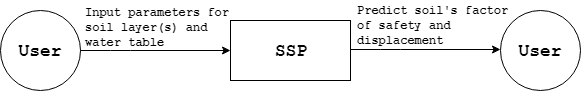
\includegraphics[width=0.6\textwidth]{SystemContextFigure.png}
		\caption{System Context}
		\label{Fig_SystemContext}
	\end{center}
\end{figure}

\noindent The responsibilities of the user and the system are as follows:

\begin{itemize}
\item User Responsibilities:
  \begin{itemize}
  \item Provide the input data related to the soil layer(s) and water table (if 
  applicable), ensuring conformation to input data format required by \progname
  \item Ensure that consistent units are used for input variables
  \item Ensure required software assumptions (Section~\ref{Assumptions}) are
    appropriate for the problem to which the user is applying the software
  \end{itemize}
\item \progname\ Responsibilities:
  \begin{itemize}
  \item Detect data type mismatch, such as a string of characters input instead
    of a floating point number
  \item Verify that the inputs satisfy the required physical constraints and 
  other data constraints (Section \ref{sec_DataConstraints})
  \item Identify the critical slip surface within the possible input range
  \item Find the factor of safety for the slope
  \item Find the interslice normal and shear forces along the critical slip 
  surface
  \end{itemize}
\end{itemize}

\subsection{User Characteristics}
\label{Sec:UserChar}
The end user of \progname\ should have an understanding of undergraduate
Level 1 Calculus and Physics, and be familiar with soil and material
properties, specifically cohesion, effective angle of friction, and unit weight.

\subsection{System Constraints} \label{sec_SystConstraints}

The Morgenstern-Price method, which involves dividing the slope into vertical 
slices, will be used to derive the equations for analysing the slope. 

\section{Specific System Description}

This section first presents the problem description, which gives a
high-level view of the problem to be solved.  This is followed by the
solution characteristics specification, which presents the
assumptions, theories, definitions and finally the instance models.

\subsection{Problem Description} \label{Sec_pd}

\progname\ is a computer program developed to evaluate the factors of safety 
for a slope's slip surfaces and identify the critical slip surface of the 
slope, as well as the interslice normal and shear forces along the critical 
slip surface. It is intended to be used as an educational tool for introducing 
slope stability issues, and to facilitate the analysis and design of a safe 
slope.

\subsubsection{Terminology and Definitions}

This subsection provides a list of terms that are used in the subsequent
sections and their meaning, with the purpose of reducing ambiguity and
 making it easier to correctly understand the requirements.

\begin{itemize}
\item {\textit{Factor of safety:} The global stability metric of a slip surface 
of a slope.}
  
\item {\textit{Slip surface:} A surface within a slope that has the potential 
to fail or displace due to load or other forces.}

\item {\textit{Critical slip surface:} Slip surface of the slope that
  has the lowest factor of safety, and is therefore most likely to
  experience failure.}

\item {\textit{Water table:} The upper boundary of a saturated zone in the 
ground.}

\item {\textit{Stress:} Force applied over an area.}
  
\item {\textit{Strain:} A measure of deformation of a body or plane under 
stress.}
  
\item {\textit{Normal force:} A force applied perpendicular to the
  plane of the material.}
  
\item {\textit{Shear force:} A force applied parallel to the plane of
  the material.}

\item {\textit{Resistive shear force:} Shear force in the direction opposite of 
the direction of potential motion, thus hindering motion along the plane.}
	
\item {\textit{Mobile shear force:} Shear force in the direction of potential 
motion, thus encouraging motion along the plane.}
	
\item {\textit{Cohesion:} An attractive force between adjacent particles that 
holds the matter together.}
  
\item {\textit{Isotropic:} A condition where the value of a property is 
independent of the direction in which it is measured.}
  
\item {\textit{Plane strain:} A condition where the resultant stresses in one 
of the directions of a 3-dimensional material can be approximated as
  0. Results when the length of one dimension of the body dominates
  the others. Stresses in the direction of the dominant dimension can be 
  approximated as 0.}

\end{itemize}

\subsubsection{Physical System Description} \label{sec_system}

The physical system of \progname{}, as shown in Figure~\ref{Fig_PhysSyst}, 
includes the following elements:

\begin{itemize}
\item[PS1:] A slope comprised of one or more layers of soil.
\item[PS2:] A water table within the soil layers, which may or may not exist.
\end{itemize}

\begin{figure}[h!]
	\begin{center}
		{
			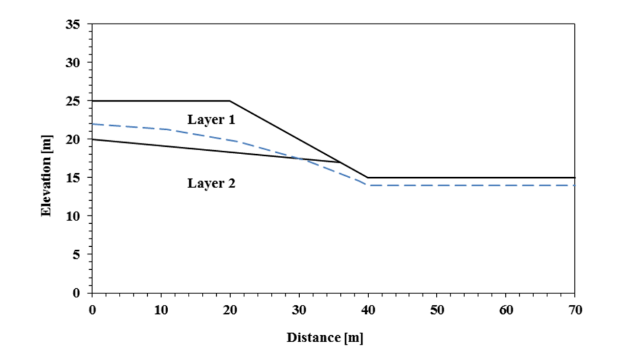
\includegraphics[width=0.7\textwidth]{PhysSyst.png}
		}
		\caption{An example slope for analysis by SSP}
		\label{Fig_PhysSyst}
	\end{center}
\end{figure}

~\newline\noindent Morgenstern-Price analysis of the slope involves 
representing the slope as a series of vertical slices. As shown in 
Figure~\ref{Fig_Index}, the index $i$ is used to denote a value for a single 
slice, and an interslice value at a given index $i$ refers to the value between 
slice $i$ and adjacent slice \textit{i+1}.

\begin{figure}[h!]
\begin{center}
{
\setlength{\unitlength}{6cm}
\begin{picture}(2,1)
% BORDER %
\thinlines
\put(0,0){\line(0,1){1}}
\put(0,1){\line(1,0){2}}
\put(2,1){\line(0,-1){1}}
\put(2,0){\line(-1,0){2}}
% SLIP SURFACE %
\linethickness{1mm}
\qbezier(0.2, 0.9)(0.5, 0.3)(1.8, 0.1)
% SLOPE %
\linethickness{0.1mm}
\put(0.1,0.9){\line(1,0){0.5}}
\put(0.6,0.9){\line(3,-2){1.2}}
\put(1.8,0.1){\line(1,0){0.1}}
% SLICES %
\put(0.2,0.9){\line(0,1){0}}
\put(0.6,0.484){\line(0,1){0.416}}
\put(0.992,0.2938){\line(0,1){0.3401}}
\put(1.4005,0.1764){\line(0,1){0.19}}
\put(1.8,0.1){\line(0,1){0}}
% interslice LABELS %
\put(0.55,0.92){$i=1$}
\put(1.3985,0.3863){$i=n-1$}
% slice LABELS %
\put(0.38,0.75){$i=1$}
\put(0.74,0.55){$i=2$}
\put(1.1,0.34){$i=n-1$}
\put(1.48,0.185){$i=n$}
\end{picture}
}
\caption{Index convention for slice and interslice values}
\label{Fig_Index}
 \end{center}
\end{figure}


~\newline\noindent A free body diagram of the forces acting on a
slice is displayed in Figure~\ref{Fig_Forces}.

\begin{figure}[h!]
\begin{center}
{
 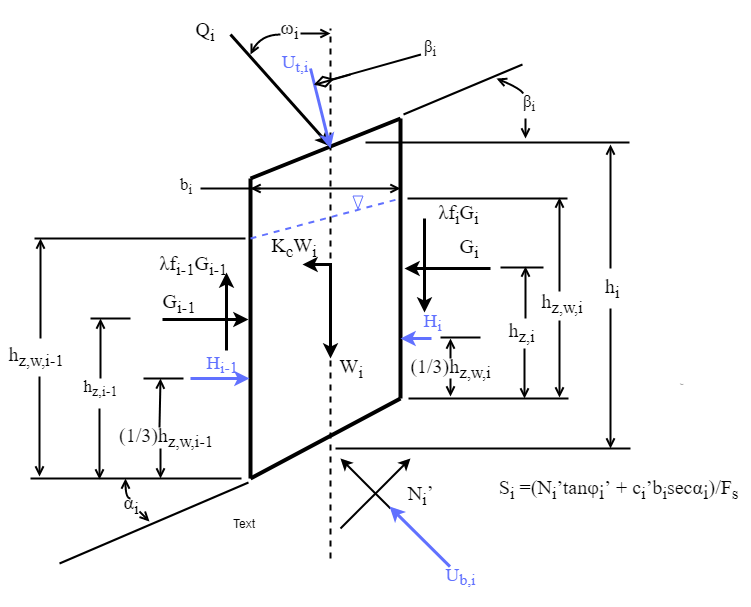
\includegraphics[width=0.7\textwidth]{ForceDiagram.png}
}
\caption{Free body diagram of forces acting on a slice}
\label{Fig_Forces}
\end{center}
\end{figure}

\subsubsection{Goal statements} \label{sec_Goals}

Given the geometry of the soil layers and water table composing the plane of a 
slope and the material properties of the layers, the goal statements are:

\begin{itemize}
\item [GS\refstepcounter{goalnum}\thegoalnum: \label{G_FS}]
  {Evaluate the factors of safety for possible slip surfaces along the slope.}
  
\item [GS\refstepcounter{goalnum}\thegoalnum: \label{G_Critical}]
  {Identify the critical slip surface for the slope, with the lowest factor of 
  safety.}

\item [GS\refstepcounter{goalnum}\thegoalnum: \label{G_Normal}]
  {Determine the interslice normal force between each pair of vertical slices   
  of the slope.}
  
\item [GS\refstepcounter{goalnum}\thegoalnum: \label{G_Shear}]
  {Determine the interslice shear force between each pair of vertical slices of 
  the slope.} 
\end{itemize}

\subsection{Solution Characteristics Specification}

The instance models that govern \progname\ are presented in
Section~\ref{sec_instance}.  The information to understand the
meaning of the instance models and their derivation is also presented,
so that the instance models can be verified.

\subsubsection{Assumptions}
\label{Assumptions}
This section simplifies the original problem and helps in developing the
theoretical models by filling in the missing information for the physical
system. The numbers given in the square brackets refer to the theoretical model
[T], general definition [GD], data definition [DD], instance model [IM], or
likely change [LC], in which the respective assumption is used.

\begin{enumerate}[label=A\arabic*:,ref={\arabic*}]
\item [A\refstepcounter{assumpnum}\theassumpnum: \label{A_Concave}] The
  slip surface is concave with respect to the slope surface. The 
  $(x_{slip},y_{slip})$ coordinates of a slip surface follow a concave up 
  function. [\iref{IM_Min}]

\item [A\refstepcounter{assumpnum}\theassumpnum: \label{A_Constant}] The factor 
of safety is assumed to be constant across a whole slip surface. 
[\dref{GD_MobShear}, \iref{IM_FS}, \iref{IM_E}]

\item [A\refstepcounter{assumpnum}\theassumpnum: \label{A_Homo}] The
  different layers of the soil are homogeneous, with consistent soil
  properties throughout. [\dref{GD_P}, \dref{GD_MobShear}, \ddref{DD_R}, 
  \ddref{DD_T}, \lcref{LC_inhomogeneous}]
  
\item [A\refstepcounter{assumpnum}\theassumpnum: \label{A_Saturated}] The soil 
properties are independent of dry or saturated conditions, with the exception 
of unit weight. [\dref{GD_P}, \dref{GD_MobShear}, \ddref{DD_R}, 
\ddref{DD_T}]

\item [A\refstepcounter{assumpnum}\theassumpnum: \label{A_Isotropic}]
  Soil layers are treated as if they have isotropic properties. [\dref{GD_P}, 
  \dref{GD_MobShear}, \ddref{DD_R}, \ddref{DD_T}]
  
\item [A\refstepcounter{assumpnum}\theassumpnum: \label{A_Base}]
  Interslice normal and shear forces have a proportional relationship,
  depending on a proportionality constant $\left({\lambda}\right)$ and an
  function $\left({f}\right)$ describing variation depending on $x$
  position. [\dref{GD_X}, \iref{IM_FS}, \iref{IM_Lambda}, \iref{IM_E}]
  
\item [A\refstepcounter{assumpnum}\theassumpnum: \label{A_2D}] The
  slope and slip surface extends far into and out of the geometry 
  ($z$-coordinate). This implies plane strain conditions, making 2D
  analysis appropriate. [\tref{TM_Eqm}]

\item [A\refstepcounter{assumpnum}\theassumpnum: \label{A_Lin}] The
  effective normal stress is large enough that the resistive shear to
  effective normal stress relationship can be approximated as a linear
  relationship. [\tref{TM_Fmc}, \dref{GD_EffNormal}]

\item [A\refstepcounter{assumpnum}\theassumpnum: \label{A_Straight}]
  The surface and base of a slice are approximated as straight lines 
  [\ddref{DD_Ub}, \ddref{DD_Ut}, \ddref{DD_Angles_alpha}, 
  \ddref{DD_Angles_Beta}, \ddref{DD_lb}, \ddref{DD_ls}].
  
\item [A\refstepcounter{assumpnum}\theassumpnum: \label{A_Seismic}] There is no 
seismic force acting on the slope. [\ddref{DD_R}, \ddref{DD_T}, \iref{IM_FS}, 
\iref{IM_Lambda}, \iref{IM_E}, \lcref{LC_Seismic}]
  
\item [A\refstepcounter{assumpnum}\theassumpnum: \label{A_External}] There is 
no imposed surface load, and therefore no external force, acting on the slope. 
[\ddref{DD_R}, \ddref{DD_T}, \iref{IM_FS}, \iref{IM_Lambda}, \iref{IM_E}, 
\lcref{LC_External}]

\end{enumerate}

\subsubsection{Theoretical Models} \label{sec_theoretical}

This section focuses on the general equations and laws that \progname\ is based
on.

~\newline

% ----------------------------- %
%        Begin TM FS           %
% ----------------------------- %
\noindent
\begin{minipage}{\textwidth}
\renewcommand*{\arraystretch}{1.5}
\begin{tabular}{| p{\colAwidth} | p{\colBwidth}|}
  
  \hline \rowcolor[gray]{0.9} Number&
  T\refstepcounter{theorynum}\thetheorynum \label{TM_FS}\\
  
  \hline Label&\bf Factor of Safety\\
  
  \hline Equation& \( \text{FS} = \frac{P}{S} \) \\
  
  \hline Description & $FS$ is the factor of safety, or stability metric of the 
  slope.\\
  & $S$ is the mobile shear force (\si{\newton\per\meter}).\\
  & $P$ is the resistive shear force (\si{\newton\per\meter}). \\
 
  \hline Source & \cite{FredlundKrahn}\\

  \hline Ref.\ By & \iref{IM_FS}, \dref{GD_MobShear} \\

  \hline
\end{tabular}
\end{minipage}\\
% ----------------------------- %
%        End TM FS              %
% ----------------------------- %

~\newline

% ----------------------------- %
%        Begin TM Equilibrium            %
% ----------------------------- %
\noindent
\begin{minipage}{\textwidth}
\renewcommand*{\arraystretch}{1.5}
\begin{tabular}{| p{\colAwidth} | p{\colBwidth}|}
  
  \hline \rowcolor[gray]{0.9} Number&
  T\refstepcounter{theorynum}\thetheorynum \label{TM_Eqm}\\
  
  \hline
  Label&\bf Static Equilibrium\\
  
  \hline Equation& \( \displaystyle\sum {F}_{\text{x}} = 
  \displaystyle\sum F_{\text{y}} = \displaystyle\sum M = 0
  \)\\

  \hline Description & For a body in static equilibrium the net
  forces and net moments acting on the body will cancel out. This equation 
  assumes a 2D space (\aref{A_2D}).\\
  & ${F_{x}}$ is the x-component of the net force (\si{\newton}).\\
  & ${F_{y}}$ is the y-component of the net force (\si{\newton}).\\
  & $M$ is the net moment (\si{\newton\meter}).\\
  
  \hline Source & \cite{FredlundKrahn}\\
  
  \hline Ref.\ By & \dref{GD_Fx}, \dref{GD_Fy}, \dref{GD_M},
  \iref{IM_Lambda} \\
  
  \hline
\end{tabular}
\end{minipage}\\
% ----------------------------- %
%        End TM Equilibrium   %
% ----------------------------- %

~\newline

% ----------------------------- %
%        Begin TM Mohr Coulomb            %
% ----------------------------- %
\noindent
\begin{minipage}{\textwidth}
\renewcommand*{\arraystretch}{1.5}
\begin{tabular}{| p{\colAwidth} | p{\colBwidth}|}
  \hline
  \rowcolor[gray]{0.9}
  Number& T\refstepcounter{theorynum}\thetheorynum \label{TM_Fmc}\\
  
  \hline Label&\bf Mohr-Coulomb Shear Strength\\
  
  \hline Equation& \( \tau = \sigma_N \cdot \tan\left( \varphi' \right) + c'
  \) \\
  
  \hline Description & The $\tau$
  versus $\sigma_N$ relationship is not truly linear, but assuming the
  effective normal force is strong enough, it can be approximated with
  a linear fit (\aref{A_Lin}), where the cohesion $c'$ represents the
  $\tau$ intercept of the fitted line.\\
  &$\tau$ is the shear strength (\si{\pascal}).\\
  &$\sigma_N$ is the normal stress (\si{\pascal}).\\
  &$\varphi$ is the effective angle of friction (\si{\degree}).\\
  &$c'$ is the effective cohesion (\si{\pascal}).\\

  \hline Source & \cite{FredlundKrahn}\\
  
  \hline Ref.\ By & \dref{GD_P}, \dref{GD_MobShear}, \ddref{DD_R},
  \ddref{DD_T}\\
  
  \hline
\end{tabular}
\end{minipage}\\
% ----------------------------- %
%        End TM Mohr Coulomb              %
% ----------------------------- %

~\newline

% ----------------------------- %
%        Begin TM Effective Stress            %
% ----------------------------- %
\noindent
\begin{minipage}{\textwidth}
\renewcommand*{\arraystretch}{1.5}
\begin{tabular}{| p{\colAwidth} | p{\colBwidth}|}
  
  \hline \rowcolor[gray]{0.9} Number&
  T\refstepcounter{theorynum}\thetheorynum \label{TM_EffStress}\\
  
  \hline Label&\bf Effective Stress\\
  
  \hline Equation& \( \sigma' =\sigma - \mu \) \\
  
  \hline Description & $\sigma$ is the total stress a soil mass needs
  to maintain itself as a rigid collection of particles (\si{\pascal}).\\
  & $\sigma'$ is the effective stress provided by the soil skeleton  
  (\si{\pascal}).\\
  & $\mu$ is the pore pressure from water within the soil (\si{\pascal}).\\

  \hline Source & \cite{FredlundKrahn}\\
  
  \hline Ref.\ By & \dref{GD_EffNormal}, \ddref{DD_R}, \iref{IM_FS},
  \iref{IM_Lambda}, \iref{IM_E}\\
  
  \hline
\end{tabular}
\end{minipage}
% ----------------------------- %
%        End TM Effective Stress             %
% ----------------------------- %

\subsubsection{General Definitions} \label{sec_gendef}

This section collects the laws and equations that will be used to build the
instance models.

~\newline

% ------------------------------------------ %
%        Begin GD Force Equilibrium X     %
% ------------------------------------------ %
\noindent
\begin{minipage}{\textwidth}
\renewcommand*{\arraystretch}{1.5}
\begin{tabular}{| p{\colAwidth} | p{\colBwidth}|}
  
  \hline \rowcolor[gray]{0.9} Number&
  GD\refstepcounter{defnum}\thedefnum \label{GD_Fx}\\
  
  \hline Label&\bf Normal Force Equilibrium\\
  \hline SI Units & \si{\newton\per\meter}\\
  
  \hline Equation& \( N_{\text{i}} \; = \begin{array}{l} \left[
      W_{\text{i}} - X_{\text{i-1}} + X_{\text{i}} +
      {U_{\text{t,i}}}\;{\cos\left(\beta_{\text{i}}\right)} +
      Q_{\text{i}}\;{\cos\left(\omega_{\text{i}}\right)}
      \right]\cos\left(\alpha_{\text{i}}\right) \\ + \left[
      {-K_{\text{c}}}\;{W_{\text{i}}} - G_{\text{i}} + G_{\text{i-1}}
      - H_{\text{i}} + H_{\text{i-1}} +
      {U_{\text{t,i}}}\;{\sin\left(\beta_{\text{i}}\right)} +
      Q_{\text{i}}\;{\sin\left(\omega_{\text{i}}\right)}
      \right]\sin\left(\alpha_{\text{i}}\right) \end{array} \) \\
 
  \hline Description & This equation satisfies \tref{TM_Eqm} in the normal 
  direction. Force equilibrium is derived from the free body diagram of 
  Figure~\ref{Fig_Forces} in section~\ref{sec_system}.\\
  &$i$ is the index representing a single slice.\\
  &$N$ is the normal force (\si{\newton\per\meter}). \\
  &$W$ is the weight (\si{\newton\per\meter}). \\
  &$X$ is the interslice shear force (\si{\newton\per\meter}). \\
  &$U_t$ is the surface hydrostatic force (\si{\newton\per\meter}). \\
  &$\beta$ is the angle between the surface of a slice and the 
  horizontal (\si{\degree}). \\
  &$Q$ is the external force (\si{\newton\per\meter}). \\
  &$\omega$ is the angle between the imposed surface load acting into 
  the surface and the vertical (\si{\degree}). \\
  &$\alpha$ is the angle between the base of a slice and the 
  horizontal (\si{\degree}). \\
  &$K_c$ is the seismic coefficient. \\
  &$G$ is the interslice normal force (\si{\newton\per\meter}). \\
  &$H$ is the interslice water force (\si{\newton\per\meter}). \\

  \hline Source & \cite{ZhuEtAl2005}\\
  
  \hline Ref.\ By & \ddref{DD_R}, \ddref{DD_T}, \iref{IM_E}\\
  
  \hline
\end{tabular}
\end{minipage}\\
% ------------------------------------------ %
%        End  GD Force Equilibrium X       %
% ------------------------------------------ %

~\newline

% ------------------------------------------ %
%        Begin GD Force Equilibrium Y     %
% ------------------------------------------ %
\noindent
\begin{minipage}{\textwidth}
\renewcommand*{\arraystretch}{1.5}
\begin{tabular}{| p{\colAwidth} | p{\colBwidth}|}
  
  \hline \rowcolor[gray]{0.9} Number&
  GD\refstepcounter{defnum}\thedefnum \label{GD_Fy}\\
  
  \hline Label&\bf Base Shear Force Equilibrium\\
  \hline SI Units & \si{\newton\per\meter}\\
  
  \hline Equation& \( S_{\text{i}} = \begin{array}{l} \left[
      W_{\text{i}} -X_{\text{i-1}} + X_{\text{i}} +
      {U_{\text{t,i}}}\;{\cos\left(\beta_{\text{i}}\right)} +
      Q_{\text{i}}\;{\cos\left(\omega_{\text{i}}\right)}
      \right]\sin\left(\alpha_{\text{i}}\right) \\ - \left[
      {-K_{\text{c}}}\;{W_{\text{i}}} - G_{\text{i}} + G_{\text{i-1}}
      - H_{\text{i}} + H_{\text{i-1}} +
      {U_{\text{t,i}}}\;{\sin\left(\beta_{\text{i}}\right)} +
      Q_{\text{i}}\;{\cos\left(\omega_{\text{i}}\right)}
      \right]\cos\left(\alpha_{\text{i}}\right) \end{array} \) \\
  
  \hline Description & This equation satisfies \tref{TM_Eqm} in the shear 
  direction. Force equilibrium is derived from the free body diagram of 
  Figure~\ref{Fig_Forces} in section~\ref{sec_system}.\\
  &$i$ is the index representing a single slice.\\
  &$S$ is the mobile shear force (\si{\newton\per\meter}). \\
  &$W$ is the weight (\si{\newton\per\meter}). \\
  &$X$ is the interslice shear force (\si{\newton\per\meter}). \\
  &$U_t$ is the surface hydrostatic force (\si{\newton\per\meter}). \\
  &$\beta$ is the angle between the surface of a slice and the 
  horizontal (\si{\degree}). \\
  &$Q$ is the external force (\si{\newton\per\meter}). \\
  &$\omega$ is the angle between the imposed surface load acting into 
  the surface and the vertical (\si{\degree}). \\
  &$\alpha$ is the angle between the base of a slice and the 
  horizontal (\si{\degree}). \\
  &$K_c$ is the seismic coefficient. \\
  &$G$ is the interslice normal force (\si{\newton\per\meter}). \\
  &$H$ is the interslice water force (\si{\newton\per\meter}). \\

  \hline Source & \cite{ZhuEtAl2005}\\
  
  \hline Ref.\ By & \ddref{DD_R}, \ddref{DD_T},\iref{IM_E}\\
  
  \hline
\end{tabular}
\end{minipage}\\
% ------------------------------------------ %
%        End  GD Force Equilibrium Y       %
% ------------------------------------------ %

~\newline

% ----------------------------- %
%        Begin GD Resistive Shear   %
% ----------------------------- %
\noindent
\begin{minipage}{\textwidth}
\renewcommand*{\arraystretch}{1.5}
\begin{tabular}{| p{\colAwidth} | p{\colBwidth}|}
  
  \hline \rowcolor[gray]{0.9} Number&
  GD\refstepcounter{defnum}\thedefnum \label{GD_P}\\
  
  \hline Label&\bf Resistive Shear Force\\
  \hline SI Units & \si{\newton\per\meter}\\
  
  \hline Equation& \( P_{\text{i}} = N'_{\text{i}} \cdot \tan\left(
  \varphi'_{\text{i}} \right) + c' \cdot \ell{}_{b,i} \) \\
  
  \hline Description & 
 The Mohr-Coulomb resistive shear strength from \tref{TM_Fmc} implemented with 
 forces.\\
 &$i$ is the index representing a single slice.\\
 &$P$ is the resistive shear force (\si{\newton\per\meter}).\\
 &$N'$ is the effective normal force (\si{\newton\per\meter}).\\
 &$\varphi'$ is the effective angle of friction (\si{\degree}).\\
 &$c'$ is the effective cohesion (\si{\pascal}).\\
 &$\ell_b$ is the width of the base of a slice in the \textit{x} direction 
 (\si{\meter}).\\

  \hline Source & \cite{ZhuEtAl2005}\\
  
  \hline Ref.\ By & \dref{GD_MobShear}, \ddref{DD_R}, \ddref{DD_T}\\
  
  \hline
\end{tabular}
\end{minipage}\\
% ----------------------------- %
%        End GD Resistive Shear             %
% ----------------------------- %

~\newline

% ----------------------------- %
%  Begin GD Mobile Shear   %
% ----------------------------- %
\noindent
\begin{minipage}{\textwidth}
\renewcommand*{\arraystretch}{1.5}
\begin{tabular}{| p{\colAwidth} | p{\colBwidth}|}
  
  \hline \rowcolor[gray]{0.9} Number&
  GD\refstepcounter{defnum}\thedefnum \label{GD_MobShear}\\
  
  \hline Label&\bf Mobile Shear Force\\
  \hline SI Units & \si{\newton\per\meter}\\
  
  \hline Equation & \( S_{\text{i}} = \frac{ P_{\text{i}} }{ \text{FS}
  } = \frac { N'_{\text{i}} \cdot \tan\left( \varphi'_{\text{i}}
    \right) + c' \cdot \ell_{b,i} }{\text{FS}} \) \\
  
  \hline Description & Mobile shear force as derived from the definition of the 
  factor of safety in \tref{TM_FS}, and the definition of $P$ in \dref{GD_P}. \\
  &$i$ is the index representing a single slice.\\
  &$S$ is the mobile shear force (\si{\newton\per\meter}).\\
  &$P$ is the resistive shear force (\si{\newton\per\meter}).\\
  &$N'$ is the effective normal force (\si{\newton\per\meter}).\\
  &$\varphi'$ is the effective angle of friction (\si{\degree}).\\
  &$c'$ is the effective cohesion (\si{\pascal}).\\
  &$\ell_b$ is the width of the base of a slice in the \textit{x} direction 
  (\si{\meter}).\\
  &$FS$ is the factor of safety.\\

  \hline Source & \cite{ZhuEtAl2005}\\
  
  \hline Ref.\ By & \ddref{DD_R}, \iref{IM_E} \\
  
  \hline
\end{tabular}
\end{minipage}\\
% ----------------------------- %
%        End GD Mobile Shear             %
% ----------------------------- %

~\newline

% ----------------------------- %
%  Begin GD Effective Normal   %
% ----------------------------- %
\noindent
\begin{minipage}{\textwidth}
	\renewcommand*{\arraystretch}{1.5}
	\begin{tabular}{| p{\colAwidth} | p{\colBwidth}|}
		
		\hline \rowcolor[gray]{0.9} Number&
		GD\refstepcounter{defnum}\thedefnum \label{GD_EffNormal}\\
		
		\hline Label&\bf Effective Normal Force\\
		\hline SI Units & \si{\newton\per\meter}\\
		
		\hline Equation & \( N'_{i} = N_{i} - U_{b,i} \) \\
	
	\hline Description & Effective normal force as derived from 
	\tref{TM_EffStress} and implemented with forces. 
	\\
	&$i$ is the index representing a single slice.\\
	&$N'$ is the effective normal force (\si{\newton\per\meter}).\\
	&$N$ is the normal force (\si{\newton\per\meter}).\\
	&$U_b$ is the base hydrostatic force (\si{\newton\per\meter}).\\
	
	\hline Source & \cite{ZhuEtAl2005}\\
	
	\hline Ref.\ By & \ddref{DD_R} \\
	
	\hline
\end{tabular}
\end{minipage}\\
% ----------------------------- %
%        End GD Effective Normal             %
% ----------------------------- %

~\newline

% ------------------------------------------ %
%        Begin GD  Interslice Normal/Shear Relationship    %
% ------------------------------------------ %
\noindent
\begin{minipage}{\textwidth}
\renewcommand*{\arraystretch}{1.5}
\begin{tabular}{| p{\colAwidth} | p{\colBwidth}|}
  
  \hline \rowcolor[gray]{0.9} Number&
  GD\refstepcounter{defnum}\thedefnum \label{GD_X}\\
  
  \hline Label&\bf Interslice Normal and Shear Force Proportionality\\
  
  \hline Equation& \( X = \lambda \cdot f \cdot
  G \) \\

  \hline Description & Mathematical representation of the primary assumption 
  for the Morgenstern-Price method (\aref{A_Base}).\\
  &$X$ is the interslice shear force (\si{\newton\per\meter}).\\
  &$G$ is the interslice normal force (\si{\newton\per\meter}).\\
  &$\lambda$ is the proportionality constant.\\
  &$f$ is a function describing variation of the interslice normal to shear 
  force ratio; can be constant or a half-sine. \\

  \hline Source & \cite{ZhuEtAl2005}\\
  
  \hline Ref.\ By & \iref{IM_FS}, \iref{IM_Lambda}, \iref{IM_E}\\
  
  \hline
\end{tabular}
\end{minipage}\\
% ------------------------------------------ %
%        End  GD Interslice Normal/Shear Relationship       %
% ------------------------------------------ %

~\newline

% ------------------------------------------ %
%        Begin GD Moment Equilibrium    %
% ------------------------------------------ %
\noindent
\begin{minipage}{\textwidth}
\renewcommand*{\arraystretch}{1.5}
\begin{tabular}{| p{\colAwidth} | p{\colBwidth}|}
  
  \hline \rowcolor[gray]{0.9} Number&
  GD\refstepcounter{defnum}\thedefnum \label{GD_M}\\
  
  \hline Label&\bf Moment Equilibrium\\
  
  \hline Equation& \( 0 = \begin{array}{l} - {G}_{\text{i}} \left[
      {z_{\text{i}}} + \frac{b_{\text{i}}}{2} {
        \tan\left(\alpha_{\text{i}}\right)} \right] + {G}_{\text{i-1}}
    \left[ {z_{\text{i-1}}} - \frac{b_{\text{i}}}{2} {
        \tan\left(\alpha_{\text{i}}\right)} \right] -
    H_{\text{i}}\left[ z_{\text{w,i}} + \frac{b_{\text{i}}}{2} {
        \tan\left(\alpha_{\text{i}}\right)} \right] \\[5pt] +
    H_{\text{i-1}}\left[ z_{\text{w,i-1}} - \frac{b_{\text{i}}}{2} {
        \tan\left(\alpha_{\text{i}}\right)} \right] +
    \frac{b_{\text{i}}}{2} \left( X_{\text{i}} + X_{\text{i-1}}
    \right) - K_{\text{c}} W_{\text{i}} \frac{h_{\text{i}}}{2} +
    U_{\text{t,i}} \sin\left(\beta_{\text{i}}\right) h_{\text{i}} \\ +
    Q_{\text{i}}\;{\sin\left(\omega_{\text{i}}\right)}
    h_{\text{i}} \end{array} \) \\

 \hline Description & This equation satisfies \tref{TM_Eqm} for the net moment. 
 Force equilibrium is derived from the free body diagram of 
 Figure~\ref{Fig_Forces} in section~\ref{sec_system}.\\
 &$i$ is the index representing a single slice.\\
 &$G$ is the interslice normal force (\si{\newton\per\meter}). \\
 &$z$ is the height in the \textit{y}-direction from the base of a slice 
 to the center of the slice (\si{\meter}).\\
 &$b$ is the width of the base of a slice in the \textit{x} direction 
 (\si{\meter}).\\
 &$\alpha$ is the angle between the base of a slice and the 
 horizontal (\si{\degree}). \\
 &$H$ is the interslice water force (\si{\newton\per\meter}). \\
 &$z_w$ is the height in the \textit{y}-direction from the base of a slice 
 halfway to the water table (\si{\meter}).\\
 &$X$ is the interslice shear force (\si{\newton\per\meter}). \\
 &$K_c$ is the seismic coefficient. \\
 &$W$ is the weight (\si{\newton\per\meter}). \\
 &$h$ is the height in the \textit{y}-direction from the base of a slice 
 to the slope surface, at the \textit{x}-direction midpoint on the slice 
 (\si{\meter}).\\
 &$U_t$ is the surface hydrostatic force (\si{\newton\per\meter}). \\
 &$\beta$ is the angle between the surface of a slice and the 
 horizontal (\si{\degree}). \\
 &$Q$ is the external force (\si{\newton\per\meter}). \\
 &$\omega$ is the angle between the imposed surface load acting into 
 the surface and the vertical (\si{\degree}). \\

  \hline Source & \cite{ZhuEtAl2005}\\
  
  \hline Ref.\ By & \iref{IM_Lambda}\\
  
  \hline
\end{tabular}
\end{minipage}\\
% ------------------------------------------ %
%        End  GD Moment Equilibrium       %
% ------------------------------------------ %

\subsubsection{Data Definition} \label{sec_datadef}

This section collects and defines all the data needed to support the general 
definitions of \ref{sec_gendef} or build the instance models of 
\ref{sec_instance}. The dimension of each quantity is also given.
~\newline

% ------------------------------------------ %
%               Begin DD W    %
% ------------------------------------------ %

\noindent
\begin{minipage}{\textwidth}
\renewcommand*{\arraystretch}{1.6}
\begin{tabular}{| p{\colAwidth} | p{\colBwidth} |}
  
\hline \rowcolor[gray]{0.9} Number&
DD\refstepcounter{datadefnum}\thedatadefnum \label{DD_W}\\

\hline Label& \bf Weight \\
\hline Symbol& $W$\\
\hline SI Units& \si{\newton\per\meter}\\

\hline
Equation & 
 $W_i$ = $b_{i}\begin{cases}
\left({y_{us,i}}-{y_{slip,i}}\right){\gamma{}_{Sat}}, & 
{y_{wt,i}}\geq{}{y_{us,i}}\\
\left({y_{us,i}}-{y_{wt,i}}\right)\gamma{}+\left({y_{wt,i}}-{y_{slip,i}}\right){\gamma{}_{Sat}},
 & {y_{us,i}}>{y_{wt,i}}>{y_{slip,i}}\\
\left({y_{us,i}}-{y_{slip,i}}\right)\gamma{}, & {y_{wt,i}}\leq{}{y_{slip,i}}
\end{cases}$
\\

\hline Description &$i$ is the index representing a single slice.\\
&$W$ is the weight (\si{\newton\per\meter}).\\
&$b$ is the width of the base of a slice in the \textit{x} direction 
(\si{\meter}).\\
&${y_{us}}$ is the \textit{y}-ordinate of a point on the slope (\si{\meter}).\\
&${y_{slip}}$ is the \textit{y}-ordinate of a point on a slip surface 
(\si{\meter}).\\
&${\gamma{}_{Sat}}$ is the soil saturated unit weight 
(\si{\newton\per\meter\cubed}).\\
&${y_{wt}}$ is the \textit{y}-ordinate of a point on the water table 
(\si{\meter}).\\
&$\gamma{}$ is the soil dry unit weight (\si{\newton\per\meter\cubed}).
\\

\hline Sources& \cite{FredlundKrahn}\\

\hline Ref.\ By & \dref{GD_Fx}, \dref{GD_Fy}, \dref{GD_M}, \ddref{DD_R}, 
\ddref{DD_T}, \iref{IM_FS}, \iref{IM_Lambda}, \iref{IM_E}\\

\hline
\end{tabular}
\end{minipage}\\

% ------------------------------------------ %
%               End DD W        %
% ------------------------------------------ %

~\newline

% ------------------------------------------ %
%               Begin DD Ub    %
% ------------------------------------------ %

\noindent
\begin{minipage}{\textwidth}
\renewcommand*{\arraystretch}{1.6}
\begin{tabular}{| p{\colAwidth} | p{\colBwidth} |}
  
\hline \rowcolor[gray]{0.9} Number&
DD\refstepcounter{datadefnum}\thedatadefnum \label{DD_Ub}\\

\hline Label& \bf Base Water Force \\
\hline Symbol& $U_b$\\
\hline SI Units& \si{\newton\per\meter}\\

\hline
Equation & 
${U_{b,i}}$ = ${\ell{}_{b,i}}\begin{cases}
\left({y_{wt,i}}-{y_{slip,i}}\right){\gamma{}_{w}}, & {y_{wt,i}}>{y_{slip,i}}\\
0, & {y_{wt,i}}\leq{}{y_{slip,i}}
\end{cases}$
\\

\hline Description &$i$ is the index representing a single slice.\\
 &${U_{b}}$ is the base hydrostatic force
 (\si{\newton\per\meter}).\\
 &${\ell{}_{b}}$ is the base length of a slice in the 
direction parallel to the slope of the base (\si{\meter}).\\
 &${y_{wt}}$ is the \textit{y}-ordinate of a point on the water table 
 (\si{\meter}).\\
 &${y_{slip}}$ is the \textit{y}-ordinate of a point on a slip surface 
 (\si{\meter}).\\
 &${\gamma{}_{w}}$ is the unit weight of water (\si{\newton\per\meter\cubed}).\\
 
\hline Sources& \cite{FredlundKrahn}\\

\hline Ref.\ By & \ddref{DD_R}, \iref{IM_FS},
\iref{IM_Lambda}, \iref{IM_E}\\

\hline
\end{tabular}
\end{minipage}\\

% ------------------------------------------ %
%               End DD Ub        %
% ------------------------------------------ %

~\newline

% ------------------------------------------ %
%               Begin DD Ut    %
% ------------------------------------------ %

\noindent
\begin{minipage}{\textwidth}
\renewcommand*{\arraystretch}{1.6}
\begin{tabular}{| p{\colAwidth} | p{\colBwidth} |}
  
\hline \rowcolor[gray]{0.9} Number&
DD\refstepcounter{datadefnum}\thedatadefnum \label{DD_Ut}\\

\hline Label& \bf Surface Hydrostatic Force \\
\hline Symbol& $U_t$\\
\hline SI Units& \si{\newton\per\meter}\\

\hline
Equation & 
${U_{t,i}}$ = ${\ell{}_{s,i}}\begin{cases}
\left({y_{wt,i}}-{y_{us,i}}\right){\gamma{}_{w}}, & {y_{wt,i}}>{y_{us,i}}\\
0, & {y_{wt,i}}\leq{}{y_{us,i}}
\end{cases}$
\\ 

\hline Description &$i$ is the index representing a single slice.\\
&${U_{t}}$ is the surface hydrostatic force (\si{\newton\per\meter}).\\
&${\ell{}_{s}}$ is the surface length of a slice in the direction 
parallel to the slope of the surface (\si{\meter}).\\
&${y_{wt}}$ is the \textit{y}-ordinate of a point on the water 
table (\si{\meter}).\\
&${y_{us}}$ is the \textit{y}-ordinate of a point on the slope (\si{\meter}).\\
&${\gamma{}_{w}}$ is the unit weight of water (\si{\newton\per\meter\cubed}).\\

\hline Sources & \cite{FredlundKrahn}\\

\hline Ref.\ By & \dref{GD_Fx}, \dref{GD_Fy}, \dref{GD_M}, \ddref{DD_R}, 
\ddref{DD_T}, \iref{IM_FS}, \iref{IM_Lambda}, \iref{IM_E}\\

\hline
\end{tabular}
\end{minipage}\\

% ------------------------------------------ %
%               End DD Ut        %
% ------------------------------------------ %

~\newline

% ------------------------------------------ %
%               Begin DD H    %
% ------------------------------------------ %

\noindent
\begin{minipage}{\textwidth}
\renewcommand*{\arraystretch}{1.6}
\begin{tabular}{| p{\colAwidth} | p{\colBwidth} |}
  
\hline \rowcolor[gray]{0.9} Number&
DD\refstepcounter{datadefnum}\thedatadefnum \label{DD_H}\\

\hline Label& \bf Interslice Water Force \\
\hline Symbol& $H$\\
\hline SI Units& \si{\newton\per\meter}\\

\hline Equation & $H_i$ = $\begin{cases}
\frac{\left[{y_{us,i}}-{y_{slip,i}}\right]^{2}}{2}{\gamma{}_{Sat}}+\left[{y_{wt,i}}-{y_{us,i}}\right]^{2}{\gamma{}_{Sat}},
 & {y_{wt,i}}\geq{}{y_{us,i}}\\
\frac{\left[{y_{wt,i}}-{y_{slip,i}}\right]^{2}}{2}{\gamma{}_{Sat}}, & 
{y_{us,i}}>{y_{wt,i}}>{y_{slip,i}}\\
0, & {y_{wt,i}}\leq{}{y_{slip,i}}
\end{cases}$
\\

\hline Description &$i$ is the index representing a single slice.\\
&$H$ is the interslice water force (\si{\newton\per\meter}).\\
&${y_{us}}$ is the \textit{y}-ordinate of a point on the slope (\si{\meter}).\\
&${y_{slip}}$ is the \textit{y}-ordinate of a point on a slip surface 
(\si{\meter}).\\
&${\gamma{}_{Sat}}$ is the soil saturated unit weight. 
(\si{\newton\per\meter\cubed}).\\
&${y_{wt}}$ is the \textit{y}-ordinate of a point on the water table 
(\si{\meter}).\\

\hline Sources & \cite{FredlundKrahn}\\

\hline Ref.\ By & \dref{GD_Fx}, \dref{GD_Fy}, \dref{GD_M}, \ddref{DD_R}, 
\ddref{DD_T}, \iref{IM_FS}, \iref{IM_Lambda}, \iref{IM_E}\\

\hline
\end{tabular}
\end{minipage}\\

% ------------------------------------------ %
%               End DD H        %
% ------------------------------------------ %

~\newline

% ------------------------------------------ %
%               Begin DD Angle Alpha   %
% ------------------------------------------ %
\noindent
\begin{minipage}{\textwidth}
\renewcommand*{\arraystretch}{1.6}
\begin{tabular}{| p{\colAwidth} | p{\colBwidth} |}
  
\hline \rowcolor[gray]{0.9} Number&
DD\refstepcounter{datadefnum}\thedatadefnum \label{DD_Angles_alpha}\\

\hline Label& \bf Base Angle\\
\hline Symbol& $\alpha$\\
\hline SI Units& \si{\degree}\\

\hline
Equation & 
\( \alpha_\text{i} = \arctan \left( \frac{y_\text{slip,i} -
  y_\text{slip,i-1}}{x_\text{slip,i} - x_\text{slip,i-1}} \right) \)\\

\hline
Description &$i$ is the index representing a single slice.\\
 &$\alpha{}$ is the angle between the base of a slice and the horizontal 
 (\si{\degree}).\\
 &${y_{slip}}$ is the \textit{y}-ordinate of a point on a slip surface 
 (\si{\meter}).\\
 &${x_{slip}}$ is the \textit{x}-ordinate of a point on a slip surface 
 (\si{\meter}).\\

\hline Sources& \cite{FredlundKrahn}\\

\hline Ref.\ By & \dref{GD_Fx}, \dref{GD_Fy}, \dref{GD_M}, \ddref{DD_lb}, 
\ddref{DD_R}, \ddref{DD_T}, \iref{IM_FS}, \iref{IM_Lambda}, \iref{IM_E}\\

\hline
\end{tabular}
\end{minipage}\\

% ------------------------------------------ %
%               End DD Angle Alpha        %
% ------------------------------------------ %

~\newline

% ------------------------------------------ %
%               Begin DD Angle Beta   %
% ------------------------------------------ %

\noindent
\begin{minipage}{\textwidth}
\renewcommand*{\arraystretch}{1.6}
\begin{tabular}{| p{\colAwidth} | p{\colBwidth} |}
  
\hline \rowcolor[gray]{0.9} Number&
DD\refstepcounter{datadefnum}\thedatadefnum \label{DD_Angles_Beta}\\

\hline Label& \bf Surface Angle \\
\hline Symbol& $\beta$\\
\hline SI Units& \si{\degree}\\

\hline
Equation & 
\( \beta_\text{i} = \arctan \left( \frac{y_\text{us,i} -
  y_\text{us,i-1}}{x_\text{us,i} - x_\text{us,i-1}} \right) \)\\

\hline
Description &$i$ is the index representing a single slice.\\
&$\beta{}$ is the angle between the surface of a slice and the 
horizontal (\si{\degree}).\\
&${y_{us}}$ is the \textit{y}-ordinate of a point on the slope (\si{\meter}).\\
&${x_{us}}$ is the \textit{x}-ordinate of a point on the slope (\si{\meter}).\\

\hline Sources& \cite{FredlundKrahn}\\

\hline Ref.\ By & \dref{GD_Fx}, \dref{GD_Fy}, \dref{GD_M}, \ddref{DD_ls}, 
\ddref{DD_R}, \ddref{DD_T}, \iref{IM_FS}, \iref{IM_Lambda}, \iref{IM_E}\\

\hline
\end{tabular}
\end{minipage}\\

% ------------------------------------------ %
%               End DD Angle Beta        %
% ------------------------------------------ %

~\newline

% ------------------------------------------ %
%               Begin DD b   %
% ------------------------------------------ %

\noindent
\begin{minipage}{\textwidth}
\renewcommand*{\arraystretch}{1.6}
\begin{tabular}{| p{\colAwidth} | p{\colBwidth} |}
  
\hline \rowcolor[gray]{0.9} Number&
DD\refstepcounter{datadefnum}\thedatadefnum \label{DD_b}\\

\hline Label& \bf Base $x$-Direction Width of a Slice \\
\hline Symbol& $b$\\
\hline SI Units& \si{\meter}\\

\hline
Equation & 
$b_i$ = ${x_{slip,i}}-{x_{slip,i-1}}$\\

\hline Description &$i$ is the index representing a single slice.\\
&$b$ is the width of the base of a slice in the \textit{x} direction 
(\si{\meter}).\\
&${x_{slip}}$ is the \textit{x}-ordinate of a point on a slip surface 
(\si{\meter}).\\

\hline Sources& \cite{FredlundKrahn}\\

\hline Ref.\ By & \dref{GD_M}, \ddref{DD_W}, \ddref{DD_lb}, \ddref{DD_ls}, 
\ddref{DD_R}, \ddref{DD_T}, \iref{IM_FS}, \iref{IM_Lambda}, \iref{IM_E}\\

\hline
\end{tabular}
\end{minipage}\\

% ------------------------------------------ %
%               End DD b   %
% ------------------------------------------ %

~\newline

% ------------------------------------------ %
%               Begin DD lb   %
% ------------------------------------------ %

\noindent
\begin{minipage}{\textwidth}
\renewcommand*{\arraystretch}{1.6}
\begin{tabular}{| p{\colAwidth} | p{\colBwidth} |}
  
\hline \rowcolor[gray]{0.9} Number&
DD\refstepcounter{datadefnum}\thedatadefnum \label{DD_lb}\\

\hline Label& \bf Total Base Length of a Slice \\
\hline Symbol& $\ell_b$\\
\hline SI Units& \si{\meter}\\

\hline
Equation & 
${\ell{}_{b,i}}$ = $b_{i}\sec\left(\alpha{}_{i}\right)$\\

\hline Description &$i$ is the index representing a single slice.\\
&${\ell{}_{b}}$ is the base length of a slice in the direction parallel to the 
slope of the base (\si{\meter}).\\
&$b$ is the width of the base of a slice in the \textit{x} direction 
(\si{\meter}).\\
&$\alpha{}$ is the angle between the base of a slice and the horizontal 
(\si{\degree}).\\

\hline Sources& \cite{FredlundKrahn}\\

\hline Ref.\ By & \dref{GD_P}, \dref{GD_MobShear}, \ddref{DD_Ub}\\

\hline
\end{tabular}
\end{minipage}\\

% ------------------------------------------ %
%               End DD lb   %
% ------------------------------------------ %

~\newline

% ------------------------------------------ %
%               Begin DD ls   %
% ------------------------------------------ %

\noindent
\begin{minipage}{\textwidth}
\renewcommand*{\arraystretch}{1.6}
\begin{tabular}{| p{\colAwidth} | p{\colBwidth} |}
  
\hline \rowcolor[gray]{0.9} Number&
DD\refstepcounter{datadefnum}\thedatadefnum \label{DD_ls}\\

\hline Label& \bf Total Surface Length of a Slice\\
\hline Symbol& $\ell_s$\\
\hline SI Units& \si{\meter}\\

\hline
Equation & 
${\ell{}_{s,i}}$ = $b_{i}\sec\left(\beta{}_{i}\right)$\\

\hline Description &$i$ is the index representing a single slice.\\
&${\ell{}_{s}}$ is the surface length of a slice in the direction parallel to 
the slope of the surface (\si{\meter}).\\
&$b$ is the width of the base of a slice in the \textit{x} direction 
(\si{\meter}).\\
&$\beta{}$ is the angle between the surface of a slice and the horizontal 
(\si{\degree}).\\

\hline Sources& \cite{FredlundKrahn}\\

\hline Ref.\ By & \ddref{DD_Ut}\\

\hline
\end{tabular}
\end{minipage}\\

% ------------------------------------------ %
%               End DD ls        %
% ------------------------------------------ %

~\newline

% ------------------------------------------ %
%               Begin DD R    %
% ------------------------------------------ %

\noindent
\begin{minipage}{\textwidth}
\renewcommand*{\arraystretch}{1.6}
\begin{tabular}{| p{\colAwidth} | p{\colBwidth} |}
  
\hline \rowcolor[gray]{0.9} Number&
DD\refstepcounter{datadefnum}\thedatadefnum \label{DD_R}\\

\hline Label& \bf Resistive Shear, Without Interslice Normal and Shear Forces \\
\hline Symbol& $R$\\
\hline SI Units& \si{\newton\per\meter}\\

\hline
Equation & 
$R_i \; = \begin{array}{l}
  \left( \begin{array}{l}
    \left[ W_{\text{i}} + U_{\text{t,i}}
      \cos\left(\beta_{\text{i}}\right) \right]
    \cos\left(\alpha_{\text{i}}\right) \\
+ \left[ - \Delta H_{\text{i}} +
  U_{\text{t,i}} \sin\left(\beta_{\text{i}}\right) \right]
\sin\left(\alpha_{\text{i}}\right) - U_{\text{b,i}} \end{array}
  \right) \cdot \tan\left(\varphi'\right)
+ c'_{\text{i}} \cdot b_{\text{i}} \cdot
\sec\left(\alpha_{\text{i}}\right) \end{array} $\\

\hline Description &$i$ is the index representing a single slice.\\
&$R$ is the resistive shear force without the influence of interslice forces
(\si{\newton\per\meter}).\\
&$W$ is the weight (\si{\newton\per\meter}).\\
&${U_{t}}$ is the surface hydrostatic force (\si{\newton\per\meter}).\\
&$\beta{}$ is the angle between the surface of a slice and the 
horizontal (\si{\degree}).\\
&$\alpha{}$ is the angle between the base of a slice and the 
horizontal (\si{\degree}).\\
&$\Delta{}H$ is the difference between interslice water forces 
(\si{\newton\per\meter}).\\
&${U_{b}}$ is the base hydrostatic force 
(\si{\newton\per\meter}).\\
&$\varphi{}'$ is the effective angle of friction (\si{\degree}).\\
&$c'$ is the effective cohesion (Pa).\\
&$b$ is the width of the base of a slice in the \textit{x} direction 
(\si{\meter}).\\

\hline Sources& \cite{ZhuEtAl2005}\\

\hline Ref.\ By & \iref{IM_FS}, \iref{IM_E}\\

\hline
\end{tabular}
\end{minipage}\\

% ------------------------------------------ %
%               End DD R         %
% ------------------------------------------ %

\subsubsection*{Resistive Shear, Without Interslice Normal and Shear Forces 
Derivation}

\noindent
The resistive shear force of a slice is defined as $P_\text{i}$ in
\dref{GD_P}, and depends upon the effective normal force.  The definition for 
normal force in \dref{GD_Fx} can be substituted into the definition for 
effective normal force in \dref{GD_EffNormal} to obtain equation~(\ref{eq:N'}).

\begin{equation} \label{eq:N'}
 N'_{\text{i}} \; = \begin{array}{l}
   \left[ W_{\text{i}} - X_{\text{i-1}} + X_{\text{i}} +
     {U_{\text{t,i}}}\;{\cos\left(\beta_{\text{i}}\right)} +
     Q_{\text{i}}\;{\cos\left(\omega_{\text{i}}\right)}
     \right]\cos\left(\alpha_{\text{i}}\right) \\ + \left[
     {-K_{\text{c}}}\;{W_{\text{i}}} - G_{\text{i}} + G_{\text{i-1}} -
     H_{\text{i}} + H_{\text{i-1}} +
     {U_{\text{t,i}}}\;{\sin\left(\beta_{\text{i}}\right)} +
     Q_{\text{i}}\;{\sin\left(\omega_{\text{i}}\right)}
     \right]\sin\left(\alpha_{\text{i}}\right) \\ -
   U_{\text{b,i}} \end{array}
 \end{equation}

\noindent
The values of the interslice forces $G$ and $X$ in the equation are
unknown. Thus, a force equilibrium without the effect of interslice normal and 
shear forces is considered, from which a value for $N^*_\text{i}$ can be 
obtained, as shown in equation~(\ref{eq:N*}).

\begin{equation} \label{eq:N*}
 N^*_{\text{i}} \; = \begin{array}{l}
   \left[ W_{\text{i}} +
     {U_{\text{t,i}}}\;{\cos\left(\beta_{\text{i}}\right)} +
     Q_{\text{i}}\;{\cos\left(\omega_{\text{i}}\right)}
     \right]\cos\left(\alpha_{\text{i}}\right) \\ + \left[
     {-K_{\text{c}}}\;{W_{\text{i}}}- H_{\text{i}} + H_{\text{i-1}} +
     {U_{\text{t,i}}}\;{\sin\left(\beta_{\text{i}}\right)} +
     Q_{\text{i}}\;{\sin\left(\omega_{\text{i}}\right)}
     \right]\sin\left(\alpha_{\text{i}}\right) -
   U_{\text{b,i}} \end{array}
\end{equation}

\noindent
Using $N^*_\text{i}$, a resistive shear force neglecting the influence
of interslice normal and shear forces can be expressed in terms of only known 
values, as shown in equation~(\ref{eq:R}).

\begin{equation*}
R_\text{i} = N^*_\text{i} \tan\left(\varphi'\right) + c'_\text{i}
\cdot b'_\text{i} \sec\left(\alpha_text{i}'\right)
\end{equation*}

\begin{equation}\label{eq:R}   R_{\text{i}} \; =
  \left( \begin{array}{l} \left[ W_{\text{i}} + U_{\text{t,i}}
      \cos\left(\beta_{\text{i}}\right) + Q_{\text{i}}
      \cos\left(\omega_{\text{i}}\right) \right]
    \cos\left(\alpha_{\text{i}}\right) \\ + \left[ - K_{\text{c}}
      W_{\text{i}} - \Delta H_{\text{i}} + U_{\text{t,i}}
      \sin\left(\beta_{\text{i}}\right) + Q_{\text{i}}
      \sin\left(\omega_{\text{i}}\right) \right]
    \sin\left(\alpha_{\text{i}}\right) - U_{\text{b,i}} \end{array}
  \right) \cdot \tan\left(\varphi'\right) + c'_{\text{i}} \cdot
  b_{\text{i}} \cdot \sec\left(\alpha_{\text{i}}\right)
 \end{equation}
 
\noindent This can be further simplified by considering assumptions 
\aref{A_Seismic} and 
\aref{A_External}, which state that the seismic coefficient and the external 
force, respectively, are 0. Removing seismic and external forces yields 
equation~(\ref{eq:Rsimple}).

\begin{equation}\label{eq:Rsimple}   R_{\text{i}} \; =
\left( \begin{array}{l} \left[ W_{\text{i}} + U_{\text{t,i}}
\cos\left(\beta_{\text{i}}\right) \right]
\cos\left(\alpha_{\text{i}}\right) \\ + \left[ - \Delta H_{\text{i}} + 
U_{\text{t,i}}
\sin\left(\beta_{\text{i}}\right) \right]
\sin\left(\alpha_{\text{i}}\right) - U_{\text{b,i}} \end{array}
\right) \cdot \tan\left(\varphi'\right) + c'_{\text{i}} \cdot
b_{\text{i}} \cdot \sec\left(\alpha_{\text{i}}\right)
\end{equation}

~\newline

% ------------------------------------------ %
%               Begin DD T    %
% ------------------------------------------ %

\noindent
\begin{minipage}{\textwidth}
\renewcommand*{\arraystretch}{1.6}
\begin{tabular}{| p{\colAwidth} | p{\colBwidth} |}
  
\hline
\rowcolor[gray]{0.9}
Number& DD\refstepcounter{datadefnum}\thedatadefnum \label{DD_T}\\

\hline
Label& \bf Mobile Shear, Without Interslice Normal and Shear Forces \\
\hline Symbol& $T$\\
\hline SI Units& \si{\newton\per\meter}\\

\hline
Equation &
$T_i$ = 
$\left(W_{i}+{U_{t,i}}\cos\left(\beta{}_{i}\right)\right)\sin\left(\alpha{}_{i}
\right)-\left(-{\Delta{}H}_{i}+{U_{t,i}}\sin\left(\beta{}_{i}\right)
\right)\cos\left(\alpha{}_{i}\right)$
\\ 

\hline Description &$i$ is the index representing a single slice.\\ 
&$T$ is the mobilized shear force without the influence of interslice forces 
(\si{\newton\per\meter}).\\
&$W$ is the weight (\si{\newton\per\meter}).\\
&${U_{t}}$ is the surface hydrostatic force (\si{\newton\per\meter}).\\ 
&$\beta{}$ is the angle between the surface of a slice and the horizontal 
(\si{\degree}).\\
&$\alpha{}$ is the angle between the base of a slice and the horizontal 
(\si{\degree}).\\
&$\Delta{}H$ is the difference between interslice water forces 
(\si{\newton\per\meter}).\\

\hline
Sources& \cite{ZhuEtAl2005}\\

\hline Ref.\ By & \iref{IM_FS}\\

\hline
\end{tabular}
\end{minipage}\\

% ------------------------------------------ %
%               End DD T         %
% ------------------------------------------ %

\subsubsection*{Mobile Shear, Without Interslice Normal and Shear Forces 
Derivation}

\noindent
The mobile shear force acting on a slice is defined as $S_\text{i}$
from the force equilibrium in \dref{GD_Fy}, also shown in
equation~(\ref{eq:Si}).

\begin{equation}  \label{eq:Si}
  S_{\text{i}} = \begin{array}{l} \left[ W_{\text{i}} -X_{\text{i-1}}
      + X_{\text{i}} +
      {U_{\text{t,i}}}\;{\cos\left(\beta_{\text{i}}\right)} +
      Q_{\text{i}}\;{\cos\left(\omega_{\text{i}}\right)}
      \right]\sin\left(\alpha_{\text{i}}\right) \\ - \left[
      {-K_{\text{c}}}\;{W_{\text{i}}} - G_{\text{i}} + G_{\text{i-1}}
      - H_{\text{i}} + H_{\text{i-1}} +
      {U_{\text{t,i}}}\;{\sin\left(\beta_{\text{i}}\right)} +
      Q_{\text{i}}\;{\cos\left(\omega_{\text{i}}\right)}
      \right]\cos\left(\alpha_{\text{i}}\right) \end{array}
\end{equation}

\noindent
The values of the interslice forces $G$ and $X$ in the equation are
unknown. Thus, a force equilibrium without the effect of interslice normal and 
shear forces is considered, from which a value for $T_i$ can be obtained, as 
shown in equation~(\ref{eq:T}).

\begin{equation}  \label{eq:T} T_{\text{i}} =
  \begin{array}{l}  
\left[ W_{\text{i}} + U_{\text{t,i}} \cos\left(\beta_{\text{i}}\right)
  + Q_{\text{i}} \cos\left(\omega_{\text{i}}\right) \right]
\sin\left(\alpha_{\text{i}}\right) \\ - \left[ - K_{\text{c}}
  W_{\text{i}} - \Delta H_{\text{i}} + U_{\text{t,i}}
  \sin\left(\beta_{\text{i}}\right) + Q_{\text{i}}
  \sin\left(\omega_{\text{i}}\right) \right]
\cos\left(\alpha_{\text{i}}\right) \end{array}
\end{equation}

\noindent
The value of $T_\text{i}$ is now defined completely in terms of known values. 
This can be further simplified by considering assumptions \aref{A_Seismic} and 
\aref{A_External}, which state that the seismic coefficient and the external 
force, respectively, are 0. Removing seismic and external forces yields 
equation~(\ref{eq:Tsimple}).

\begin{equation}  \label{eq:Tsimple} T_{\text{i}} =
\begin{array}{l}  
\left[ W_{\text{i}} + U_{\text{t,i}} \cos\left(\beta_{\text{i}}\right) \right]
\sin\left(\alpha_{\text{i}}\right) - \left[ - \Delta H_{\text{i}} + 
U_{\text{t,i}}
\sin\left(\beta_{\text{i}}\right) \right]
\cos\left(\alpha_{\text{i}}\right) \end{array}
\end{equation}

~\newline

\subsubsection{Instance Models} \label{sec_instance}

This section transforms the problem defined in the
Section~\ref{Sec_pd} into one which is expressed in mathematical
terms. It uses concrete symbols defined in Section~\ref{sec_datadef}
to replace the abstract symbols in the models identified in the
Sections~\ref{sec_theoretical} and ~\ref{sec_gendef}.

~\newline\noindent The goals \gsref{G_FS}, \gsref{G_Normal}, and 
\gsref{G_Shear} are met by the simultaneous solution of \iref{IM_FS}, 
\iref{IM_Lambda}, and \iref{IM_E}. The goal \gsref{G_Critical} is met by
\iref{IM_Min}.

~\newline\noindent The Morgenstern-Price Method is a vertical slice,
limit equilibrium slope stability analysis method. Analysis is
performed by breaking the assumed slip surface into a series of
vertical slices of mass. Static equilibrium analysis is performed, using two 
force equations and one moment equation as in \tref{TM_Eqm}. The problem
is statically indeterminate with only these 3 equations and one
constitutive equation (the Mohr-Coulomb shear strength of
\tref{TM_Fmc}), so the assumption \aref{A_Base} and corresponding equation 
\dref{GD_X} are used. The force equilibrium equations can be modified to be 
expressed only in terms of known physical values, as done in \ddref{DD_R} and 
\ddref{DD_T}.

~\newline

% ------------------------------------------ %
%               Begin IM Factor of safety      %
% ------------------------------------------ %

\noindent
\begin{minipage}{\textwidth}
\renewcommand*{\arraystretch}{1.6}
\begin{tabular}{| p{\colAwidth} | p{\colBwidth} |}
  
\hline \rowcolor[gray]{0.9} Number&
IM\refstepcounter{instnum}\theinstnum \label{IM_FS}\\

\hline Label& \bf Factor of Safety \\

\hline Input & ${\Psi_{\text{c}}}$ , ${\Phi_{\text{c}}}$ ,
${T_{\text{i}}}$ , ${R_{\text{i}}}$ \\

\hline
Output &
\( {FS}= \frac{\displaystyle\sum_{i=1}^{n-1} \left[ {R_{i}}
    \;{\displaystyle\prod_{c=i}^{n-1} \frac{\Psi_{c}}{\Phi_{c}}
    }\right] + {R_{n}} }{\displaystyle\sum_{i=1}^{n-1} \left[ {T_{i}}
    \;{\displaystyle\prod_{c=i}^{n-1} \frac{\Psi_{c}}{\Phi_{c}}
    }\right] + {T_{n}} } \)\\

\hline Description & $i$ is the index representing a single slice.\\
&$n$ is the total number of slices.\\
&$FS$ is the factor of safety.\\
&$R$ is the resistive shear force  without the influence of interslice forces 
(\si{\newton\per\meter}).\\
&$\Psi$ is the second constant used to convert shear without the 
influence of interslice forces to shear with the influence of 
interslice forces.\\
&$\Phi$ is the first constant used to convert shear without the 
influence of interslice forces to shear with the influence of 
interslice forces.\\
&$T$ is the mobile shear force  without the influence of interslice forces 
(\si{\newton\per\meter}).\\

\hline Sources& \cite{ZhuEtAl2005}\\

\hline Ref.\ By & \iref{IM_Lambda}, \iref{IM_E}\\

\hline
\end{tabular}
\end{minipage}\\

% ------------------------------------------ %
%               End IM Factor of Safety         %
% ------------------------------------------ %

\subsubsection*{Factor of Safety Derivation}

\noindent
Using the boundary conditions from \iref{IM_E} that $G_{\text{0}}$ and 
$G_{\text{n}}$ are equal to $0$, one can derive equation~(\ref{eq:FS}),
also seen in \iref{IM_FS}.

\begin{equation}\label{eq:FS}
 {FS}= \frac{\displaystyle\sum_{i=1}^{n-1} \left[ {R_{i}}
 	\;{\displaystyle\prod_{c=i}^{n-1} \frac{\Psi_{c}}{\Phi_{c}}
 	}\right] + {R_{n}} }{\displaystyle\sum_{i=1}^{n-1} \left[ {T_{i}}
 	\;{\displaystyle\prod_{c=i}^{n-1} \frac{\Psi_{c}}{\Phi_{c}}
 	}\right] + {T_{n}} }\\
\end{equation}

\noindent
The constants $\Psi$ and $\Phi$, described in equations \ref{eq:Psi}
and \ref{eq:Phi} of the derivation for \iref{IM_E}, are functions of the 
unknowns: the interslice normal and shear force proportionality constant, 
$\lambda$ 
(\iref{IM_Lambda}), and the factor of safety, $FS$ (\iref{IM_FS}).

~\newline

% ------------------------------------------ %
%               Begin IM Lambda      %
% ------------------------------------------ %

\noindent
\begin{minipage}{\textwidth}
\renewcommand*{\arraystretch}{1.6}
\begin{tabular}{| p{\colAwidth} | p{\colBwidth} |}
  
\hline \rowcolor[gray]{0.9} Number&
IM\refstepcounter{instnum}\theinstnum \label{IM_Lambda}\\

\hline Label& \bf Normal and Shear Force Proportionality Constant \\

\hline Input & $b_{\text{i}}$ , $G_{\text{i}}$ , $H_{\text{i}}$ ,
$\alpha_{\text{i}}$ , $h_{\text{i}}$ , $W_{\text{i}}$ ,
$U_{\text{t,i}}$ , $\beta_{\text{i}}$ , $f_{\text{i}}$ \\

\hline
Output & 
\( {C1_{\text{i}}}= \) 
\(  \left\{
\renewcommand{\arraystretch}{2}
\begin{tabular}{ p{6.5cm} r} 
  $ {{b}_{\text{1}}}\left[{{G}_{\text{1}} + {H}_{\text{1}}}
    \right]{\tan\left(\alpha_{\text{1}}\right) } $ &  $
  \text{i}={\text{1}} $ \\
\noindent\parbox[c]{\hsize} {$ {{b}_{\text{i}}} \left[
    \left({{G}_{\text{i}} + {G}_{\text{i-1}}}\right) +
    \left({{H}_{\text{i}} + {H}_{\text{i-1}}}\right)
    \right]{\tan\left(\alpha_{\text{i}}\right)} \\ +
  {{h}_{\text{i}}}\left( 
  -{2}\;{U_{\text{t,i}}}\;{\sin\left(\beta_{\text{i}}\right)}
  \;\right) $}
&  $ 2\leq\text{i}\leq{\text{n-1}} $ \\ $
                {{b}_{\text{n}}}\left[{{G}_{\text{n-1}} +
                    {H}_{\text{n-1}}}\right]{\tan\left(\alpha_{\text{n-1}}\right)
                } $ &  $ \text{i}=\text{n} $ \\
\end{tabular} 
\renewcommand{\arraystretch}{1}
\right. \)
~\newline~\newline
\( {C2_{\text{i}}}= \)
\(  \left\{
\renewcommand{\arraystretch}{2}
\begin{tabular}{ p{6.5cm} r} 
  $ {{b}_{\text{1}}}{{G}_{\text{1}}}{f_{\text{1}}} $ &  $
  \text{i}=\text{1} $ \\ $ {{b}_{\text{i}}}\;{\left({
      {f_{\text{i}}}{{G}_{\text{i}}} +
      {f_{\text{i-1}}}{{G}_{\text{i-1}}} }\right)} $ &  $
  2\leq\text{i}\leq{\text{n-1}} $ \\ $
  {{b}_{\text{n}}}{{G}_{\text{n-1}}}{f_{\text{n-1}}} $ &  $
  \text{i}=\text{n} $ \\
\end{tabular} 
\renewcommand{\arraystretch}{1}
\right. \) 
~\newline
\( \lambda= \frac{ \displaystyle\sum_{i=1}^{n} {C1_{\text{i}}}}
   {\displaystyle\sum_{i=1}^{n} {C2_{\text{i}}}} \) \\

\hline Description & $i$ is the index representing a single slice.\\
&$n$ is the total number of slices.\\
&$b$ is the width of the base of a slice in the \textit{x} direction 
(\si{\meter}).\\
&$G$ is the interslice normal force (\si{\newton\per\meter}).\\
&$H$ is the interslice water force (\si{\newton\per\meter}). \\
&$\alpha$ is the angle between the base of a slice and the 
horizontal (\si{\degree}). \\
&$h$ is the height in the \textit{y}-direction from the base of a slice 
to the slope surface, at the \textit{x}-direction midpoint on the slice 
(\si{\meter}).\\
&$U_t$ is the surface hydrostatic force (\si{\newton\per\meter}).\\
&$\beta$ is the angle between the surface of a slice and the 
horizontal (\si{\degree}). \\
&$f$ is a function describing variation of the interslice normal to shear 
force ratio; can be constant or a half-sine. \\
&$\lambda$ is the proportionality constant.\\

\hline Sources& \cite{ZhuEtAl2005}\\

\hline Ref.\ By & \iref{IM_FS}, \iref{IM_E} \\

\hline
\end{tabular}
\end{minipage}\\

% ------------------------------------------ %
%               End IM Lambda         %
% ------------------------------------------ %

\subsubsection*{Normal/Shear Force Ratio Derivation}

 From the moment equilibrium of \dref{GD_M}, with the primary assumption for 
 the Morgenstern-Price method of \aref{A_Base} and associated definition 
 \dref{GD_X}, equation~(\ref{eq:Moment}) can be derived.

\begin{equation}\label{eq:Moment}
  0 = \begin{array}{l} - {G}_{\text{i}} \left[ {z_{\text{i}}} -
      \frac{b_{\text{i}}}{2} { \tan\left(\alpha_{\text{i}}\right)}
      \right] + {G}_{\text{i-1}} \left[ {z_{\text{i-1}}} +
      \frac{b_{\text{i}}}{2} { \tan\left(\alpha_{\text{i}}\right)}
      \right] - H_{\text{i}}\left[ z_{\text{w,i}} -
      \frac{b_{\text{i}}}{2} { \tan\left(\alpha_{\text{i}}\right)}
      \right] \\[5pt] + H_{\text{i-1}}\left[ z_{\text{w,i-1}} +
      \frac{b_{\text{i}}}{2} { \tan\left(\alpha_{\text{i}}\right)}
      \right] -\lambda \frac{b_{\text{i}}}{2} \left( G_{\text{i}}
    f_{\text{i}} + G_{\text{i-1}} f_{\text{i-1}} \right) +
    K_{\text{c}} W_{\text{i}} \frac{h_{\text{i}}}{2} - U_{\text{t,i}}
    \sin\left(\beta_{\text{i}}\right) h_{\text{i}} -
    Q_{\text{i}}\;{\sin\left(\omega_{\text{i}}\right)}
    h_{\text{i}} \end{array}
\end{equation} 

\noindent
Rearranging the equation in terms of $\lambda$ leads to 
equation~(\ref{eq:lambda1}).

\begin{equation}\label{eq:lambda1}
  \lambda = \frac { \begin{array}{l} - {G}_{\text{i}} \left[
        {z_{\text{i}}} - \frac{b_{\text{i}}}{2} {
          \tan\left(\alpha_{\text{i}}\right)} \right] +
      {G}_{\text{i-1}} \left[ {z_{\text{i-1}}} +
        \frac{b_{\text{i}}}{2} { \tan\left(\alpha_{\text{i}}\right)}
        \right] - H_{\text{i}}\left[ z_{\text{i}} -
        \frac{b_{\text{i}}}{2} { \tan\left(\alpha_{\text{i}}\right)}
        \right] \\[5pt] + H_{\text{i-1}}\left[ z_{\text{i-1}} +
        \frac{b_{\text{i}}}{2} { \tan\left(\alpha_{\text{i}}\right)}
        \right] + K_{\text{c}} W_{\text{i}} \frac{h_{\text{i}}}{2} -
      U_{\text{t,i}} \sin\left(\beta_{\text{i}}\right) h_{\text{i}} -
      Q_{\text{i}}\;{\sin\left(\omega_{\text{i}}\right)}
      h_{\text{i}} \end{array} } { \frac{b_{\text{i}}}{2} \left[
      G_{\text{i}} f_{\text{i}} + G_{\text{i-1}} f_{\text{i-1}}
      \right] }
\end{equation}

\noindent
Taking the summation of all slices, considering the boundary
conditions that $G_{\text{0}}$ and $G_{\text{n}}$ are equal to zero, and 
removing the seismic and external forces due to \aref{A_Seismic} and 
\aref{A_External}, respectively, a general equation for the constant $\lambda$ 
is developed in equation~(\ref{eq:Lambda}), also found in \iref{IM_Lambda}.

\begin{equation}\label{eq:Lambda}
\lambda= \frac{ \displaystyle\sum_{i=1}^{n} { {b_{\text{i}}} \left[
      \left({{G}_{\text{i}} + {G}_{\text{i-1}}}\right) +
      \left({{H}_{\text{i}} + {H}_{\text{i-1}}}\right)
      \right]{\tan\left(\alpha_{\text{i}}\right)} \\ +
    {{h}_{\text{i}}}\;\left[ 
    -{2}\;{U_{\text{t,i}}}\;{\sin\left(\beta_{\text{i}}\right)} \right] }}
         {\displaystyle\sum_{i=1}^{n} { {{b}_{\text{i}}}\;{\left[{
                   {f_{i}}{{G}_{\text{i}}} +
                   {f_{\text{i-1}}}{{G}_{\text{i-1}}} }\right]} }}
\end{equation}

\noindent
Equation~(\ref{eq:Lambda}) for $\lambda$, is a function of the unknown
interslice normal force $G$ (\iref{IM_E}).

~\newline

% ------------------------------------------ %
%               Begin IM E    %
% ------------------------------------------ %

\noindent
\begin{minipage}{\textwidth}
\renewcommand*{\arraystretch}{1.6}
\begin{tabular}{| p{\colAwidth} | p{\colBwidth} |}
  
\hline \rowcolor[gray]{0.9} Number&
IM\refstepcounter{instnum}\theinstnum \label{IM_E}\\

\hline Label& \bf Interslice Normal Forces \\

\hline Input & $\text{FS}$, $T_\text{i}$, $R_\text{i}$, $\Psi_i$,
$\Phi_i$\\

\hline
Output &

\( G_{\text{i}}= \) 
\(  \left\{
\renewcommand{\arraystretch}{1.75}
\begin{tabular}{ p{3cm} l} 
$ \frac{ \left(\text{FS}\right) T_{\text{1}} - R_{\text{1}} }{
    \Phi_{\text{i}} } $ &  $\text{i=1}$ \\
\noindent\parbox[c]{\hsize} {$ \frac{ \Psi_{\text{i-1}} \cdot
    G_{\text{i-1}} + \left(\text{FS}\right) \cdot T_{\text{i}} -
    R_{\text{i}} }{ \Phi_{\text{i}} } $} & 
$2\leq\text{i}\leq\text{n-1}$ \\
\noindent\parbox[c]{\hsize} {$0 $} &  $\text{i=0}$ $\vee$ $\text{i=n}$
\end{tabular}
\renewcommand{\arraystretch}{1}
\right. \) \\

\hline Description & $i$ is the index representing a single slice.\\
&$n$ is the total number of slices.\\
&$G$ is the interslice normal force (\si{\newton\per\meter}).\\
&$FS$ is the factor of safety.\\
&$T$ is the mobile shear force  without the influence of interslice forces 
(\si{\newton\per\meter}).\\
&$R$ is the resistive shear force  without the influence of interslice forces 
(\si{\newton\per\meter}).\\
&$\Phi$ is the first constant used to convert shear without the 
influence of interslice forces to shear with the influence of 
interslice forces.\\
&$\Psi$ is the second constant used to convert shear without the 
influence of interslice forces to shear with the influence of 
interslice forces.\\


\hline Sources& \cite{ZhuEtAl2005}\\

\hline Ref.\ By & \iref{IM_FS}, \iref{IM_Lambda}\\

\hline
\end{tabular}
\end{minipage}\\

% ------------------------------------------ %
%               End IM E         %
% ------------------------------------------ %

\subsubsection*{Interslice Force Derivation} \label{sec:Ederivation}

Substituting the normal force equilibrium of \dref{GD_Fx} and the assumption 
\aref{A_Base} represented by \dref{GD_X} into the effective normal force 
definition from \dref{GD_EffNormal} yields equation~(\ref{eq:F_perp}).

\begin{equation}\label{eq:F_perp}   N'_{\text{i}}  = \begin{array}{l}    
    \left[ W_{\text{i}} - \lambda \cdot f_{\text{i-1}} \cdot
      G_{\text{i-1}} + \lambda \cdot f_{\text{i}} \cdot G_{\text{i}} +
      U_{\text{t,i}} {\cos\left(\beta_{\text{i}}\right)} +
      Q_{\text{i}} \cos\left(\omega_{\text{i}}\right)
      \right]\cos\left(\alpha_{\text{i}}\right) \\ + \left[
      -K_{\text{c}} W_{\text{i}} - G_{\text{i}} + G_{\text{i-1}} -
      H_{\text{i}} + H_{\text{i-1}} + U_{\text{t,i}}
      \sin\left(\beta_{\text{i}}\right) + Q_{\text{i}}
      \sin\left(\omega_{\text{i}}\right) \right]
    \sin\left(\alpha_{\text{i}}\right) - U_{\text{b,i}} \end{array}
\end{equation}

\noindent
Next, substituting the base shear force equilibrium of \dref{GD_Fy} and the 
assumption of \dref{GD_X} into the definition of mobilized shear from 
\dref{GD_MobShear} results in equation~(\ref{eq:F_par}).

\begin{equation}  \label{eq:F_par}
  \frac{
   N'_{\text{i}} \tan\left(\varphi'\right._{i}) + c'_{\text{i}} \cdot 
   b'_{\text{i}} \cdot \sec\left(\alpha_{\text{i}}\right.) 
  }
    { \text{FS} }
     = \begin{array}{l}
      \left[ W_{\text{i}}
       - \lambda \cdot
    
      f_{\text{i-1}} \cdot G_{\text{i-1}} + \lambda \cdot f_{\text{i}}
      \cdot G_{\text{i}} + U_{\text{t,i}}
      \cos\left(\beta_{\text{i}}\right) + Q_{\text{i}}
      \cos\left(\omega_{\text{i}}\right) \right]
    \sin\left(\alpha_{\text{i}}\right) \\ - \left[ -K_{\text{c}}
      W_{\text{i}} - G_{\text{i}} + G_{\text{i-1}} - H_{\text{i}} +
      H_{\text{i-1}} + U_{\text{t,i}} \cdot
      \sin\left(\beta_{\text{i}}\right) + Q_{\text{i}}
      \sin\left(\omega_{\text{i}}\right) \right]
    \cos\left(\alpha_{\text{i}}\right) \end{array}
\end{equation}

\noindent
Substituting equation~(\ref{eq:F_perp}), \ddref{DD_R}, and \ddref{DD_T} into 
equation~(\ref{eq:F_par}) and rearranging results in 
equation~(\ref{eq:Interslice1})

\begin{equation}\label{eq:Interslice1}
G_\text{i} \left[ \begin{array}{l} \left[ \lambda \cdot f_\text{i}
      \cos\left(\alpha_\text{i}\right) -
      \sin\left(\alpha_\text{i}\right) \right]
    \tan\left(\varphi'\right._{i}) \\ - \left[ \lambda \cdot f_\text{i}
      \sin\left(\alpha_\text{i}\right) +
      \cos\left(\alpha_\text{i}\right) \right.]
    \left(\text{FS}\right) \end{array} \right] = G_\text{i-1}
\left[ \begin{array}{l} \left[ \lambda \cdot f_\text{i-1}
      \cos\left(\alpha_\text{i}\right) -
      \sin\left(\alpha_\text{i}\right) \right]
    \tan\left(\varphi'\right._{i}) 
    \\ - \left[ \lambda \cdot f_\text{i-1}
      \sin\left(\alpha_\text{i}\right) +
      \cos\left(\alpha_\text{i}\right) \right]
    \left(\text{FS}\right) \end{array} \right] +
\left(\text{FS}\right) \cdot T_\text{i} - R_\text{i}
\end{equation}

\noindent
Where $R$ and $T$ are the resistive and mobile shear
of the slice, without the influence of interslice forces $G$ and $X$,
as defined in \ddref{DD_R} and \ddref{DD_T}. The constants $\Phi$ and $\Psi$ 
are defined below in equations~(\ref{eq:Phi}) and~(\ref{eq:Psi}) 
respectively.

\begin{equation}\label{eq:Phi} \begin{aligned}
\Phi_{\text{i}}={} & \left[ \lambda \cdot f_{\text{i}}
  \cos\left(\alpha_{\text{i}}\right) -
  \sin\left(\alpha_{\text{i}}\right) \right]\left[
  \tan\left({\varphi'_{\text{i}}}\right) \right] - \left[ \lambda
  \cdot f_{\text{i}} \sin\left(\alpha_{\text{i}}\right) +
  \cos\left(\alpha_{\text{i}}\right) \right]\left(\text{FS}\right)
\end{aligned}\end{equation}

~\newline 
\begin{equation}\label{eq:Psi}\begin{aligned}
\Psi_{\text{i}} ={}& \left[ \lambda \cdot f_{\text{i}}
  \cos\left(\alpha_{\text{i+1}}\right) -
  \sin\left(\alpha_{\text{i+1}}\right) \right]\left[
  \tan\left(\varphi'\right) \right] - \left[ \lambda \cdot
  f_{\text{i}} \sin\left(\alpha_{\text{i+1}}\right) +
  \cos\left(\alpha_{\text{i+1}}\right) \right] \left( \text{FS}
\right)
 \end{aligned}\end{equation}

~\newline
\noindent These constants can be used to simplify 
equation~(\ref{eq:Interslice1}) to obtain equation~(\ref{eq:Interslice2}), 
which can be found in \iref{IM_E}.

\begin{equation}\label{eq:Interslice2}
{G}_{\text{i}} = \frac{{\Psi_{\text{i-1}}}\;{{G}_{\text{i-1}}} +
  \left({{FS}}\right)\;{T_{\text{i}}} -
       {R_{\text{i}}}}{\Phi_{\text{i}}}
\end{equation}

\noindent
The constants $\Psi$ and $\Phi$ in equation~(\ref{eq:Interslice2}) for
are functions of the unknowns: the proportionality constant, $\lambda{}$  
(\iref{IM_Lambda}), and the factor of safety, $FS$ (\iref{IM_FS}).

~\newline

% ------------------------------------------ %
%               Begin IM Minimization    %
% ------------------------------------------ %

\noindent
\begin{minipage}{\textwidth}
\renewcommand*{\arraystretch}{1.6}
\begin{tabular}{| p{\colAwidth} | p{\colBwidth} |}
  
\hline \rowcolor[gray]{0.9} Number&
IM\refstepcounter{instnum}\theinstnum \label{IM_Min}\\

\hline Label& \bf Critical Slip Surface Identification \\

\hline Input & $\{(x_\text{us},y_\text{us})\}$ \\

\hline Output & \(  \left( \text{FS}_\text{Min}, \left\{ 
\left(x_\text{cs},y_\text{cs}\right)\right\} \right)
 = \Upsilon\left( \left\{\left(x_\text{us},y_\text{us}\right)\right\} \right)\)
 \\

\hline Description & $FS_{Min}$ is the minimum factor of safety associated with 
the critical slip surface.\\
&$x_{cs}$ is the \textit{x}-ordinate of a point on the critical slip surface 
(\si{\meter}).\\
&$x_{cs}$ is the \textit{y}-ordinate of a point on the critical slip surface 
(\si{\meter}).\\
&$\Upsilon$ is a minimization algorithm or function.\\
&$x_{us}$ is the \textit{x}-ordinate of a point on the slope (\si{\meter}).\\
&$y_{us}$ is the \textit{y}-ordinate of a point on the slope (\si{\meter}).\\

\hline Sources& \cite{LiEtAl}\\

\hline
\end{tabular}
\end{minipage}\\

% ------------------------------------------ %
%               End IM Minimization         %
% ------------------------------------------ %

\bmac{Should this IM exist? It doesn't arise from any T}

\wss{We need something to explain that we pick the slip surface with the minimum
  factor of safety.  I'll give this some further thought on whether this is the
  best way to say it.}

\subsubsection{Data Constraints} \label{sec_DataConstraints}    

Tables~\ref{TblInputVar} and \ref{TblOutputVar} show the data constraints on 
the input and output variables, respectively. The column for physical 
constraints gives the physical limitations on the range of values that can be 
taken by the variable. The uncertainty column provides an estimate of the 
confidence with which the physical quantities can be measured. This information 
would be part of the input if one were performing an uncertainty quantification 
exercise. The constraints are conservative, to give the user of the model the 
flexibility to experiment with unusual situations. The column of typical values 
is intended to provide a feel for a common scenario.

\newpage

\begin{table}[!h]
\caption{Input Variables} 
\renewcommand{\arraystretch}{1.5}
\noindent \begin{longtable*}{p{3.1cm} p{5.1cm} p{1.2cm} c}
  \toprule  \label{TblInputVar}
  \textbf{Var} & \textbf{Physical Constraints} & \textbf{Typical
    Value} & \textbf{Uncertainty}\\ \midrule
  $\{(x_{wt},y_{wt})\}$ (*) & At least two ordered pairs must be specified. 
  Starts and ends on the same $x$ values as soil layers.  
  & N/A & 10\% \\
  $\{(x_{slip},y_{slip})\}$ for potential slip surface entry and exit points & 
  $x$ values must be between the minimum and maximum $x$ values of the slope. & 
  N/A & 10\% \\
  $\{(x_{us},y_{us})\}$ (**) & At least two ordered pairs must be specified. 
  $y$ values of consecutive vertices are always increasing or always 
  decreasing. All layers start and end on the same $x$ values. & N/A & 10\% \\
  $c'$ (**) & $c >0$ & 10 & 10\%\\
  $\varphi'$ (**) & $ 0 < \varphi < 90 $ & 25 & 10\% \\
  $\gamma$ (**) & $\gamma > 0$ & 20 & 10\% \\
  $\gamma_{\text{Sat}}$ (**) & $\gamma_{\text{Sat}} > 0 $ & 20 & 10\% \\
  $\gamma_{\text{w}}$ & $\gamma_{\text{w}} > 0 $ & 9.8 & 10\% \\
  \bottomrule
\end{longtable*}
\end{table}

\noindent \begin{description}
\item[(*)] Optional input.
\item[(**)] Input must be specified for each layer.
\end{description}

\begin{table}[!h]
\caption{Output Variables} 
\renewcommand{\arraystretch}{1.2} 
\noindent \begin{longtable*}{p{2cm} p{14cm}} 
  \toprule \label{TblOutputVar}
  \textbf{Var} & \textbf{Physical Constraints} \\
  \midrule 
  $FS$ & $FS>0$ \\
  $\{(x_{cs},y_{cs})\}$ &  $x$ values must be between the minimum and maximum 
  $x$ values of the slope. $y$ values must not exceed the maximum $y$ value of 
  the slope. The slope between consecutive vertices must be always increasing 
  as $x$ increases. \\
  $G_i$ & $G_i>0$ \\
  $X_i$ & $X_i<0$ \\
  \bottomrule
\end{longtable*}
\end{table}

\subsubsection{Properties of a Correct Solution} \label{sec_CorrectSolution}

\noindent
A correct solution must exhibit conformation to the system of non-linear 
equations presented in \iref{IM_FS}, \iref{IM_Lambda}, and \iref{IM_E}. In 
addition, the factor of safety for the critical slip surface must be lower than 
the factors of safety calculated for other slip surfaces compared by 
\iref{IM_Min}. The coordinates of the critical slip surface must form a concave 
up function.

\wss{It seems to me that the content of this section could all be deleted,
  except for the last sentence.  Saying that the solution agrees with the
 instance models is covered by the requirements.  The shape of the critical slip
 surface seems to be the only new information here.  What do you think BM?}

\bmac{I agree that the information is covered elsewhere. Even the last sentence 
is mostly covered by \aref{A_Concave}. I struggled to come up with content for 
this section.}

\section{Requirements} \label{sec_Reqs}

This section provides the functional requirements, the business tasks
that the software is expected to complete, and the nonfunctional
requirements, the qualities that the software is expected to exhibit.

\subsection{Functional Requirements}

\noindent \begin{itemize}


\item[R\refstepcounter{reqnum}\thereqnum \label{R_Inputs}:] Read the
  inputs, shown in the table below, and store the data.
  \begin{table}[!h]
  \renewcommand{\arraystretch}{1.5}
  \noindent \begin{tabularx}{1.0\textwidth}{l l X} \toprule \textbf{symbol} &
%  \noindent \begin{longtable}{l l p{12cm}} \toprule \textbf{symbol} &
    \refstepcounter{tablenum}  \label{Table:Inputs}
    \textbf{unit} & \textbf{description}\\ \midrule
    $\left(x,y\right)$ & $\text{m}$ & $x$ and $y$-coordinates for vertices
    of the slope layers, for the water table if one exists, and for potential 
    entry and exit points of a slip surface.\\
    $c'$ & $\si{\pascal}$ & Cohesion for each slope layer. \\
    $\varphi'$ & \si{\degree} & Effective angle of friction for each
    slope layer. \\
    $\gamma$ & $\si{\newton\per\meter\cubed}$ & Unit weight of dry
    soil for each slope layer. \\
    $\gamma_{\text{Sat}}$ & $\si{\newton\per\meter\cubed}$ & Unit
    weight of saturated soil for each slope layer. \\
    $\gamma_{\text{w}}$ & $\si{\newton\per\meter\cubed}$ & Unit
    weight of water. \\
    N/A & N/A & A boolean decision on which form of the interslice variation 
    function \textit{f} the user desires: constant or half-sine.\\ \bottomrule
\end{tabularx}
\end{table}

\item[R\refstepcounter{reqnum}\thereqnum \label{R_KinAdm}:] Verify that the 
input data lies within physical constraints shown in Table~\ref{TblInputVar}.

\item[R\refstepcounter{reqnum}\thereqnum \label{R_InitGen}:] Generate
potential critical slip surfaces for the input slope (using \iref{IM_Min}). 

\item[R\refstepcounter{reqnum}\thereqnum \label{R_FS}:] Calculate the
  factors of safety for each of the potential critical slip surfaces (using 
  \iref{IM_FS}, \iref{IM_Lambda}, and \iref{IM_E}).

\item[R\refstepcounter{reqnum}\thereqnum \label{R_Minimize}:] Compare the 
factor of safety for each potential critical slip surface to determine the 
minimum factor of safety, corresponding to the critical slip surface (using 
\iref{IM_Min}).

\item[R\refstepcounter{reqnum}\thereqnum \label{R_VerifyOutput}:] Verify that 
the factor of safety, critical slip surface, and interslice forces satisfy the 
physical constraints shown in Table~\ref{TblOutputVar} and Section
\ref{sec_CorrectSolution}.

\item[R\refstepcounter{reqnum}\thereqnum \label{R_CritGraph}:] Display
  the critical slip surface of the 2D slope, as determined from \iref{IM_Min}, 
  graphically. 
  
\item[R\refstepcounter{reqnum}\thereqnum \label{R_OutputFS}:] Display the value 
of the factor of safety for the critical slip surface, as determined from 
\iref{IM_FS}, \iref{IM_Lambda}, and \iref{IM_E}.

\item[R\refstepcounter{reqnum}\thereqnum \label{R_NormalGraph}:] Using 
\iref{IM_FS}, \iref{IM_Lambda}, and \iref{IM_E}, calculate and 
graphically display the interslice normal forces.

\item[R\refstepcounter{reqnum}\thereqnum \label{R_ShearGraph}:] Using 
\iref{IM_FS}, \iref{IM_Lambda}, and \iref{IM_E}, calculate and 
graphically display the interslice shear forces.
  
\end{itemize}


\subsection{Nonfunctional Requirements}

\progname\ is intended to be an educational tool, therefore accuracy and
performance speed are secondary program priorities. Instead, the following 
non-functional requirements are prioritized:

\begin{itemize}
\item[NFR1:] Correctness, achieved if the outputs of the code have the 
properties described 
in \ref{sec_CorrectSolution}.
\item[NFR2:] Understandability, achieved if the code is modularized with 
complete module guide and module interface specification.
\item[NFR3:] Reusability, achieved if the code is modularized.
\item[NFR4:] Maintainability, achieved if the traceability between 
requirements, assumptions, theoretical models, general definitions, data 
definitions, instance models, likely changes, and modules is completely 
recorded in traceability matrices in the SRS and module guide.
\end{itemize}

\section{Likely Changes}

\noindent \begin{itemize}
\item[\refstepcounter{lcnum}\lthelcnum \label{LC_inhomogeneous}:] The system 
currently assumes the different layers of the soil are homogeneous 
(\aref{A_Homo}). In the future, implementation can be added for inconsistent 
soil properties throughout.
 
\item[\refstepcounter{lcnum}\lthelcnum \label{LC_Seismic}:] The system 
currently assumes no seismic force (\aref{A_Seismic}). In the future, 
implementation can be added for the presence of seismic force.

\item[\refstepcounter{lcnum}\lthelcnum \label{LC_External}:] The system 
currently assumes no external force (\aref{A_External}).
In the future, implementation can be added for an imposed surface load on the 
slope.
\end{itemize}

\section{Unlikely Changes}
If changes were to be made with regard to the following,
a different algorithm would be needed.

\begin{itemize}
\item[\refstepcounter{ucnum}\ltheucnum \label{UC_insf}:] Changes related to 
\aref{A_Base} are not possible due to the dependency of the calculations on the 
proportional relationship between interslice normal and shear forces.
\item[\refstepcounter{ucnum}\ltheucnum \label{UC_inhomogeneous}:] \aref{A_2D} 
allows for 2D analysis with these models only because stress along 
$z$-direction is zero. These models do not take into account stress in the 
$z$-direction, and therefore cannot be used without manipulation to attempt 
3-dimensional analysis.
\end{itemize}

\bmac{This section is not on the template, not sure if it should be kept}

\wss{I'm going to think about adding this section to the template.  It is a way
  to show that some of the assumptions are critical to the identity of the
  problem.}

\section{Traceability Matrices and Graphs}

The purpose of the traceability matrices is to provide easy references on what
has to be additionally modified if a certain component is changed.  Every time a
component is changed, the items in the column of that component that are marked
with an ``X'' may have to be modified as well.  Tables~\ref{Table:trace} 
and~\ref{Table:trace2} show the dependencies of theoretical models, general 
definitions, data definitions, and instance models with each other. 
Table~\ref{Table:R_trace} shows the dependencies of instance models, 
requirements, and data constraints on each other. Table~\ref{Table:A_trace} 
shows the dependencies of theoretical models, general definitions, data 
definitions, instance models, and likely changes on the assumptions.

\setlength{\tabcolsep}{6pt}

\begin{table}[h!]
\centering
\begin{tabular}{|c|c|c|c|c|c|c|c|c|c|c|c|}
\hline
& \aref{A_Concave}& \aref{A_Constant}& \aref{A_Homo}& \aref{A_Saturated}&
\aref{A_Isotropic}& \aref{A_Base}& \aref{A_2D}& \aref{A_Lin}& 
\aref{A_Straight}& \aref{A_Seismic}& \aref{A_External} \\
\hline
\tref{TM_FS}            & & & & & & & & & & & \\ \hline
\tref{TM_Eqm}           & & & & & & & X& & & & \\ \hline
\tref{TM_Fmc}           & & & & & & & & X& & & \\ \hline
\tref{TM_EffStress}     & & & & & & & & & & & \\ \hline
\dref{GD_Fx}            & & & & & & & & & & & \\ \hline
\dref{GD_Fy}            & & & & & & & & & & & \\ \hline
\dref{GD_P}             & & & X& X& X& & & & & & \\ \hline
\dref{GD_MobShear}      & & X& X& X& X& & & & & & \\ \hline
\dref{GD_EffNormal}     & & & & & & & & X& & & \\ \hline
\dref{GD_X}             & & & & & & X& & & & & \\ \hline
\dref{GD_M}             & & & & & & & & & & & \\ \hline
\ddref{DD_W}            & & & & & & & & & & & \\ \hline
\ddref{DD_Ub}           & & & & & & & & & X& & \\ \hline
\ddref{DD_Ut}           & & & & & & & & & X& & \\ \hline
\ddref{DD_H}            & & & & & & & & & & & \\ \hline
\ddref{DD_Angles_alpha} & & & & & & & & & X& & \\ \hline
\ddref{DD_Angles_Beta}  & & & & & & & & & X& & \\ \hline
\ddref{DD_b}            & & & & & & & & & & & \\ \hline
\ddref{DD_lb}           & & & & & & & & & X& & \\ \hline
\ddref{DD_ls}           & & & & & & & & & X& & \\ \hline
\ddref{DD_R}            & & & X& X& X& & & & & X& X\\ \hline
\ddref{DD_T}            & & & X& X& X& & & & & X& X\\ \hline
\iref{IM_FS}            & & X& & & & X& & & & X& X\\ \hline
\iref{IM_Lambda}        & & & & & & X& & & & X& X\\ \hline
\iref{IM_E}             & & X& & & & X& & & & X& X\\ \hline
\iref{IM_Min}           & X& & & & & & & & & & \\ \hline
\lcref{LC_inhomogeneous}& & & X& & & & & & & & \\ \hline
\lcref{LC_Seismic}      & & & & & & & & & & X& \\ \hline
\lcref{LC_External}     & & & & & & & & & & & X\\
\hline
\end{tabular}
\caption{Traceability Matrix Showing the Connections Between Assumptions 
and Other Items}
\label{Table:A_trace}
\end{table}

\afterpage{
\begin{landscape}
\begin{table}[h!]
\centering
\begin{tabular}{|c|c|c|c|c|c|c|c|c|c|c|c|}
\hline        
& \tref{TM_FS}& \tref{TM_Eqm}& \tref{TM_Fmc}& \tref{TM_EffStress}&
\dref{GD_Fx}& \dref{GD_Fy} & \dref{GD_P}& \dref{GD_MobShear}& 
\dref{GD_EffNormal}& \dref{GD_X}& \dref{GD_M} \\
\hline
\tref{TM_FS}            & & & & & & & & & & & \\ \hline
\tref{TM_Eqm}           & & & & & & & & & & & \\ \hline
\tref{TM_Fmc}           & & & & & & & & & & & \\ \hline
\tref{TM_EffStress}     & & & & & & & & & & & \\ \hline
\dref{GD_Fx}            & & X& & & & & & & & & \\ \hline
\dref{GD_Fy}            & & X& & & & & & & & & \\ \hline
\dref{GD_P}             & & & X& X& & & & & & & \\ \hline
\dref{GD_MobShear}      & X& & X& X& & & X& & & & \\ \hline
\dref{GD_EffNormal}     & & & & X& & & & & & & \\ \hline
\dref{GD_X}             & & & & & & & & & & & \\ \hline
\dref{GD_M}             & & X& & & & & & & & & \\ \hline
\ddref{DD_W}            & & & & & & & & & & & \\ \hline
\ddref{DD_Ub}           & & & & & & & & & & & \\ \hline
\ddref{DD_Ut}           & & & & & & & & & & & \\ \hline
\ddref{DD_H}            & & & & & & & & & & & \\ \hline
\ddref{DD_Angles_alpha} & & & & & & & & & & & \\ \hline
\ddref{DD_Angles_Beta}  & & & & & & & & & & & \\ \hline
\ddref{DD_b}            & & & & & & & & & & & \\ \hline
\ddref{DD_lb}           & & & & & & & & & & & \\ \hline
\ddref{DD_ls}           & & & & & & & & & & & \\ \hline
\ddref{DD_R}            & & & X& X& X& X& X& X& X& & \\ \hline
\ddref{DD_T}            & & & X& X& X& X& X& & & & \\ \hline
\iref{IM_FS}            & X& & & X& & & & & & X& \\ \hline
\iref{IM_Lambda}        & & X& & X& & & & & & X& X \\ \hline
\iref{IM_E}             & & & & X& X& X& & X& & X& \\ \hline
\iref{IM_Min}           & & & & & & & & & & & \\
\hline
\end{tabular}
\caption{Traceability Matrix Showing the Connections Between Items of Different 
Sections With Theory Models and General Definitions}
\label{Table:trace}
\end{table}
\end{landscape}
}

\afterpage{
\begin{landscape}
\begin{table}[h!]
\centering
\begin{tabular}{|c|c|c|c|c|c|c|c|c|c|c|c|c|c|c|c|}
\hline        
& \ddref{DD_W}& \ddref{DD_Ub}& \ddref{DD_Ut}& \ddref{DD_H}& 
\ddref{DD_Angles_alpha}& \ddref{DD_Angles_Beta}& \ddref{DD_b}& \ddref{DD_lb}& 
\ddref{DD_ls}& \ddref{DD_R}& \ddref{DD_T}& \iref{IM_FS}& \iref{IM_Lambda}& 
\iref{IM_E}& \iref{IM_Min} \\
\hline
\tref{TM_FS}            & & & & & & & & & & & & & & & \\ \hline
\tref{TM_Eqm}           & & & & & & & & & & & & & & & \\ \hline
\tref{TM_Fmc}           & & & & & & & & & & & & & & & \\ \hline
\tref{TM_EffStress}     & & & & & & & & & & & & & & & \\ \hline
\dref{GD_Fx}            & X& & X& X& X& X& & & & & & & & & \\ \hline
\dref{GD_Fy}            & X& & X& X& X& X& & & & & & & & & \\ \hline
\dref{GD_P}             & & & & & & & & X& & & & & & & \\ \hline
\dref{GD_MobShear}      & & & & & & & & X& & & & & & & \\ \hline
\dref{GD_EffNormal}     & & & & & & & & & & & & & & & \\ \hline
\dref{GD_X}             & & & & & & & & & & & & & & & \\ \hline
\dref{GD_M}             & X& & X& X& X& X& X& & & & & & & & \\ \hline
\ddref{DD_W}            & & & & & & & & & & & & & & & \\ \hline
\ddref{DD_Ub}           & & & & & & & & X& & & & & & & \\ \hline
\ddref{DD_Ut}           & & & & & & & & & X& & & & & & \\ \hline
\ddref{DD_H}            & & & & & & & & & & & & & & & \\ \hline
\ddref{DD_Angles_alpha} & & & & & & & & & & & & & & & \\ \hline
\ddref{DD_Angles_Beta}  & & & & & & & & & & & & & & & \\ \hline
\ddref{DD_b}            & & & & & & & & & & & & & & & \\ \hline
\ddref{DD_lb}           & & & & & X& & X& & & & & & & & \\ \hline
\ddref{DD_ls}           & & & & & & X& X& & & & & & & & \\ \hline
\ddref{DD_R}            & X& X& X& X& X& X& X& & & & & & & & \\ 
\hline
\ddref{DD_T}            & X& & X& X& X& X& X& & & & & & & & \\ 
\hline
\iref{IM_FS}            & X& X& X& X& X& X& X& & & X& X& & X& X& \\ 
\hline
\iref{IM_Lambda}        & X& X& X& X& X& X& X& & & & & X& & X& \\ 
\hline
\iref{IM_E}             & X& X& X& X& X& X& X& & & X& & X& X& & \\ 
\hline
\iref{IM_Min}           & & & & & & & & & & & & & & & \\
\hline
\end{tabular}
\caption{Traceability Matrix Showing the Connections Between Items of Different 
	Sections with Data Definitions and Instance Models}
\label{Table:trace2}
\end{table}
\end{landscape}
}

\begin{table}[h!]
\centering
\begin{tabular}{|c|c|c|c|c|c|c|}
\hline
& \iref{IM_FS}& \iref{IM_Lambda}& \iref{IM_E}& \iref{IM_Min}& 
\ref{sec_DataConstraints} & \rref{R_Inputs}\\
\hline
\iref{IM_FS}          & & & & & & X\\ \hline
\iref{IM_Lambda}      & & & & & & X\\ \hline
\iref{IM_E}           & & & & & & X\\ \hline
\iref{IM_Min}         & & & & & & X\\ \hline 
\rref{R_Inputs}       & & & & & & \\ \hline
\rref{R_KinAdm}       & & & & & X& \\ \hline
\rref{R_InitGen}      & & & & X& & \\ \hline
\rref{R_FS}           & X& X& X& & & \\ \hline 
\rref{R_Minimize}     & & & & X& & \\ \hline
\rref{R_VerifyOutput} & & & & & X& \\ \hline
\rref{R_CritGraph}    & & & & & X& \\ \hline
\rref{R_OutputFS}     & X& X& X& & & \\ \hline
\rref{R_NormalGraph}  & X& X& X& & & \\ \hline
\rref{R_ShearGraph}   & X& X& X& & & \\
\hline
\end{tabular}
\caption{Traceability Matrix Showing the Connections Between Requirements and 
Instance Models}
\label{Table:R_trace}
\end{table}
%
%Below is the large traceability matrix before it was split into 2, in case it 
%is desired to make it 1 again
%
%\afterpage{
%	\begin{landscape}
%		\begin{table}[h!]
%			\centering
%			
%\begin{tabular}{|c|c|c|c|c|c|c|c|c|c|c|c|c|c|c|c|c|c|c|c|c|c|c|c|c|c|c|c|c|}
%				\hline        
%				& \tref{TM_FS}& \tref{TM_Eqm}& \tref{TM_Fmc}& 
%\tref{TM_EffStress}&
%				\dref{GD_Fx}& \dref{GD_Fy} & \dref{GD_P}& \dref{GD_MobShear}& 
%\dref{GD_X}& 
%				\dref{GD_M}& \ddref{DD_W}& \ddref{DD_Ub}& \ddref{DD_Ut}& 
%\ddref{DD_H}& 
%				\ddref{DD_Angles_alpha}& \ddref{DD_Angles_Beta}& \ddref{DD_b}& 
%\ddref{DD_lb}& 
%				\ddref{DD_ls}& \ddref{DD_Kc}& \ddref{DD_Q}& \ddref{DD_EX}& 
%\ddref{DD_R}& 
%				\ddref{DD_T}& \iref{IM_FS}& \iref{IM_Lambda}& \iref{IM_E}& 
%\iref{IM_Min} \\
%				\hline
%				\tref{TM_FS}            & & & & & & & & & & & & & & & & & & & & 
%& & & & & & & & 
%				\\ \hline
%				\tref{TM_Eqm}           & & & & & & & & & & & & & & & & & & & & 
%& & & & & & & & 
%				\\ \hline
%				\tref{TM_Fmc}           & & & & & & & & & & & & & & & & & & & & 
%& & & & & & & & 
%				\\ \hline
%				\tref{TM_EffStress}     & & & & & & & & & & & & & & & & & & & & 
%& & & & & & & & 
%				\\ \hline
%				\dref{GD_Fx}            & & X& & & & & & & & & & & & & & & & & 
%& & & & & & & & 
%				& \\ \hline
%				\dref{GD_Fy}            & & X& & & & & & & & & & & & & & & & & 
%& & & & & & & & 
%				& \\ \hline
%				\dref{GD_P}             & & & X& X& & & & & & & & & & & & & & & 
%& & & & & & & & 
%				& \\ \hline
%				\dref{GD_MobShear}      & X& & X& X& & & X& & & & & & & & & & & 
%& & & & & & & & 
%				& & \\ \hline
%				\dref{GD_X}             & & & & & & & & & & & & & & & & & & & & 
%& & & & & & & & 
%				\\ \hline
%				\dref{GD_M}             & & X& & & & & & & & & & & & & & & & & 
%& & & & & & & & 
%				& \\ \hline
%				\ddref{DD_W}            & & & & & & & & & & & & & & & & & & & & 
%& & & & & & & & 
%				\\ \hline
%				\ddref{DD_Ub}           & & & & & & & & & & & & & & & & & & & & 
%& & & & & & & & 
%				\\ \hline
%				\ddref{DD_Ut}           & & & & & & & & & & & & & & & & & & & & 
%& & & & & & & & 
%				\\ \hline
%				\ddref{DD_H}            & & & & & & & & & & & & & & & & & & & & 
%& & & & & & & & 
%				\\ \hline
%				\ddref{DD_Angles_alpha} & & & & & & & & & & & & & & & & & & & & 
%& & & & & & & & 
%				\\ \hline
%				\ddref{DD_Angles_Beta}  & & & & & & & & & & & & & & & & & & & & 
%& & & & & & & & 
%				\\ \hline
%				\ddref{DD_b}            & & & & & & & & & & & & & & & & & & & & 
%& & & & & & & & 
%				\\ \hline
%				\ddref{DD_lb}           & & & & & & & & & & & & & & & & & & & & 
%& & & & & & & & 
%				\\ \hline
%				\ddref{DD_ls}           & & & & & & & & & & & & & & & & & & & & 
%& & & & & & & & 
%				\\ \hline
%				\ddref{DD_Kc}           & & & & & & & & & & & & & & & & & & & & 
%& & & & & & & & 
%				\\ \hline
%				\ddref{DD_Q}            & & & & & & & & & & & & & & & & & & & & 
%& & & & & & & & 
%				\\ \hline
%				\ddref{DD_EX}           & & & & & & & & & & & & & & & & & & & & 
%& & & & & & & & 
%				\\ \hline
%				\ddref{DD_R}            & & & X& X& X& X& X& X& X& & X& X& X& 
%X& X& X& X& X& X& 
%				X& X& X& & & & & & \\ \hline
%				\ddref{DD_T}            & & & X& X& X& X& X& X& X& & X& X& X& 
%X& X& X& X& X& X& 
%				X& & & & & & & & \\ \hline
%				\iref{IM_FS}            & X& & & & & & & & X& & X& X& X& X& X& 
%X& X& X& X& X& 
%				X& X& X& X& & X& X& \\ \hline
%				\iref{IM_Lambda}        & & X& & & & & & & X& X& X& X& X& X& X& 
%X& X& X& X& X& 
%				X& X& & & X& & X& \\ \hline
%				\iref{IM_E}             & & & & X& X& X& & & X& & X& X& X& X& 
%X& X& X& X& X& X& 
%				X& X& & & X& X& & \\ \hline
%				\iref{IM_Min}           & & & & & & & & & & & & & & & & & & & & 
%& & & & & & & & 
%				\\
%				\hline
%			\end{tabular}
%			\caption{Traceability Matrix Showing the Connections Between Items 
%of Different 
%				Sections}
%			\label{Table:trace}
%		\end{table}
%	\end{landscape}
%}

The purpose of the traceability graphs is also to provide easy references on
what has to be additionally modified if a certain component is changed.  The
arrows in the graphs represent dependencies. The component at the tail of an
arrow is depended on by the component at the head of that arrow. Therefore, if a
component is changed, the components that it points to should also be
changed. Figure~\ref{Fig_ATrace} shows the dependencies of theoretical models,
general definitions, data definitions, instance models, likely changes, and
assumptions on each other. Figure~\ref{Fig_RTrace} shows the dependencies of
instance models, requirements, and data constraints on each other.

\begin{figure}[h!]
	\begin{center}
		%\rotatebox{-90}
		{
			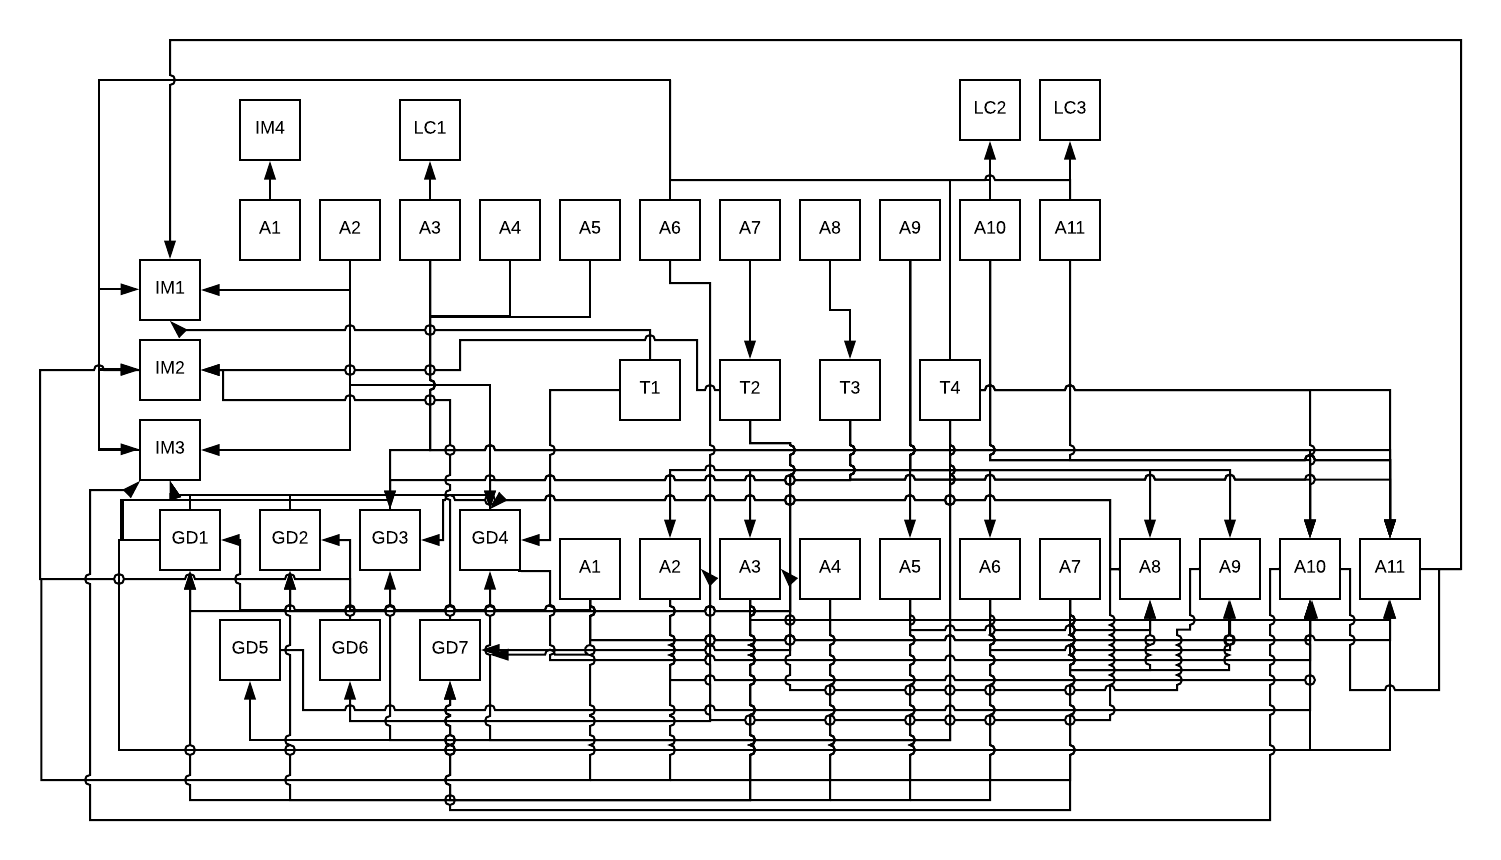
\includegraphics[width=\textwidth]{ATrace.png}
		}
		\caption{\label{Fig_ATrace} Traceability Matrix Showing the Connections 
		Between Items of Different Sections}
	\end{center}
\end{figure}


\begin{figure}[h!]
	\begin{center}
		%\rotatebox{-90}
		{
			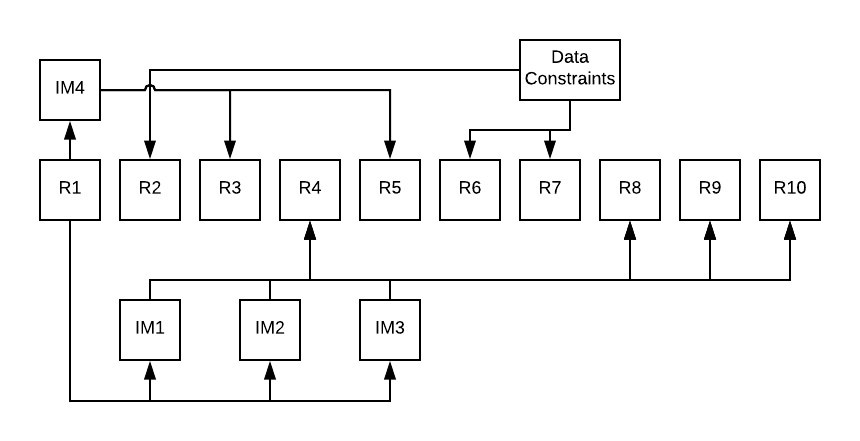
\includegraphics[width=0.7\textwidth]{RTrace.png}
		}
		\caption{\label{Fig_RTrace} Traceability Matrix Showing the Connections 
		Between Requirements, Instance Models, and Data Constraints}
	\end{center}
\end{figure}

\newpage

\bibliographystyle {plain}
\bibliography {../../refs/References}

\section{Appendix}

\subsection{Symbolic Parameters}
There are no symbolic parameters.

\end{document}
